% Caption index paper, ACL 2027 (ARR) long paper. Ported from docs/paper/caption_index_draft.md (v1.2, 2026-10-26).
% Sections still in bullets in the draft are lists here. Build: latexmk -pdf caption_index.tex
\documentclass[11pt]{article}

\usepackage[review]{acl}
\usepackage{times}
\usepackage{latexsym}
\usepackage[T1]{fontenc}
\usepackage[utf8]{inputenc}
\usepackage{microtype}
\usepackage{inconsolata}
\usepackage{graphicx}
\usepackage{booktabs}
\usepackage{amsmath}
\usepackage{xcolor}
\usepackage{listings}
\lstset{basicstyle=\ttfamily\scriptsize, breaklines=true, columns=fullflexible, keepspaces=true,
  frame=single, framesep=3pt, xleftmargin=4pt, xrightmargin=4pt}

\graphicspath{{../figures/}}

% The draft's characters, so numbers can be written as in the Markdown source.
\DeclareUnicodeCharacter{2212}{\ensuremath{-}}
\DeclareUnicodeCharacter{2248}{\ensuremath{\approx}}
\DeclareUnicodeCharacter{2264}{\ensuremath{\le}}
\DeclareUnicodeCharacter{2265}{\ensuremath{\ge}}
\DeclareUnicodeCharacter{00D7}{\ensuremath{\times}}
\DeclareUnicodeCharacter{2192}{\ensuremath{\to}}
\DeclareUnicodeCharacter{00B1}{\ensuremath{\pm}}
\DeclareUnicodeCharacter{03BA}{\ensuremath{\kappa}}
\DeclareUnicodeCharacter{03C1}{\ensuremath{\rho}}
\DeclareUnicodeCharacter{03C4}{\ensuremath{\tau}}
\DeclareUnicodeCharacter{221E}{\ensuremath{\infty}}

\newcommand{\qbe}{\ensuremath{Q_{\mathrm{BE}}}}
\newcommand{\pending}[1]{\textbf{\textcolor{red}{[PENDING: #1]}}}
\newcommand{\draftnote}[1]{\textcolor{blue}{[#1]}}
\newcommand{\cl}{cl.}

\title{Caption Once, Ask Cheaply: What a Question-Blind Caption Index\\Buys a Video Reader}

\author{Anonymous submission}

\begin{document}
\maketitle

\begin{abstract}
Captions written once per video window, without the questions, can serve as an index from which a cheaper text reader answers later questions. We ask when such an index lets a reader answer better than it does from the frames, why, and at what cost. The captioner sees exactly the reader's frames, which splits the effect of captions into source, visual budget, captioner and modality effects. On 297 TempCompass questions, in the pre-registered main test, Gemini's captions of the reader's frames raise a Claude Haiku reader's accuracy by 0.15 over Haiku's self-captions, its own captions of the same frames. In follow-ups, each predicted in writing before it ran, the gain is 0.08 at matched visual tokens, 0.06 with Claude Sonnet captioning identical input, and 0.13 for an open-weights reader (Qwen2.5-VL-7B). Turning frames into text does not help by itself: Haiku gains +0.03 from its self-captions (CI up to +0.09), and Sonnet and Qwen lose 0.09 and 0.12. The index pays through the cheaper reader: Haiku on a stronger captioner's index costs 1/23 to 1/26 of Sonnet on frames per question, repays the captioning within 1.2--3.7 questions per video (1.4--6.3 without the CLI's fixed prompt), and is 0--9 points less accurate. When a reader keeps both, a rule fixed in advance from the question's aspect and the reader and captioner predicts, on 738 new questions, whether the index or the frames will be right where they disagree (AUC 0.67); no question-blind score of the video or of its captions improves it. On unmanipulated videos, Sonnet's question-blind self-captions keep 0.95 of the gain its frames give over the question alone. The losses sit in the benchmark's built stress tests: question-blind captions lose the comparison between two copies of a clip shown at once, and the direction of reversed clips; 61--73\% of wrong answers come from captions that do not decide the question.
\end{abstract}

\section{Introduction}

Many video question answering systems first caption the video and then reason over the text \citep{llovi,videotree,silvr}. When the captions are written once and reused for every later question, they act as an index: captioning is paid once, and each question costs only a text read. Recent work builds such indexes for long video \citep{cfd,capmem,sprout}; in CapMem, a model's own captions beat its frames only on videos over 20 minutes. Two questions remain open. First, when a reader answers better from captions than from frames, the reason is unclear. The captioner may have seen more of the video, spent more visual tokens, or been a stronger model, or text may be easier for the reader than pixels. Second, whether the index pays depends on the full cost per question and on the one-time cost of captioning.

We hold the information fixed. The captioner receives exactly the frames the reader would see. A caption made from these frames cannot contain information about the video that the frames lack (Proposition~1), so an accuracy gain from captions is information that the reader can use more easily, not new information. Arms that change one thing at a time then split the effect of captions into four parts: the source the captioner sees (the video or the reader's frames), the visual tokens it spends, the captioner model, and the modality (a reader's self-captions against its frames). We use two model families: Claude Haiku and Sonnet read, and Haiku, Sonnet and Gemini caption. An open-weights model, Qwen2.5-VL-7B, reads the main arms and captions for itself. The data are 297 multiple-choice questions from TempCompass \citep{tempcompass}, on videos with a median length of 10\,s. The main test was pre-registered on a separate development set, and each follow-up was logged with a predicted value before it ran.

The captioner matters; the modality does not. With Haiku reading, Gemini's captions of the reader's frames beat Haiku's self-captions by 0.15 (the pre-registered test), and by 0.08 at matched visual tokens; Sonnet's captions of identical input give 0.06. Haiku is no more accurate on its self-captions than on the frames they describe (+0.03, CI up to +0.09; −0.06 on 738 further questions about the same videos), and Sonnet is 0.09 less accurate on its own. An open-weights reader (Qwen2.5-VL-7B, greedy decoding) replicates both. Two pre-registered predictions failed: Haiku was expected to lose on its self-captions (−0.08), and captions to lose direction and speed more than other aspects. On the four indexes Sonnet wrote, Haiku and Sonnet read equally well, although Sonnet reads frames 0.19 better; on Gemini's captions Sonnet reads 0.05 more. The saving comes from a cheaper reader, at 0 to 9 points of accuracy. The losses are concentrated: on unmanipulated videos, Sonnet on its self-captions is within 0.01 of its frames. When two copies of a clip play at different speeds, question-blind captions do not say which is faster, although the same model, shown the question, often sees it; on reversed clips they describe the forward event or state no direction. Where the index and the frames disagree, which one is right is predicted by the question's aspect and the model pair; scores of the video's motion, its cuts or how well the captions cover the frames add nothing, and a rule frozen on the confirmatory questions holds on new ones.

Our contributions are:
\begin{enumerate}
\item A decomposition of the effect of captions into source, visual budget, captioner and modality effects, with arms that change one thing each, in two model families (\S\ref{sec:effects}).
\item A pre-registered test, with exploratory replications within one model family at identical input and with an open-weights reader: the captioner effect is positive, and the modality effect at most +0.09 (\S\ref{sec:captioner}--\ref{sec:modality}, \S\ref{sec:robust}).
\item A cost account per question from input, output and thinking tokens, and the break-even number of questions per video, also projected to longer videos (\S\ref{sec:cost}).
\item An account of what question-blind captions lose, from minimal pairs, a question-aware control and an audit of wrong answers (\S\ref{sec:types}--\ref{sec:aware}).
\item A decision rule for when to read the index instead of the frames, chosen on the confirmatory questions and tested on 738 new ones, and a null result for question-blind video and caption scores as predictors (\S\ref{sec:decide}).
\end{enumerate}
The study is limited to short videos, multiple-choice questions and one benchmark.

\section{Setup}

\subsection{Task and data}
\label{sec:data}
We use TempCompass's multiple-choice questions \citep{tempcompass} on five aspects: action, speed, direction, order and attribute change. A development set of 100 questions set the hypotheses. The confirmatory set samples 60 questions per aspect, one per video, on videos the development set does not use; 297 remain after an amendment (Appendix~\ref{app:amend}). TempCompass builds most of its videos to defeat shortcuts, so we report four video types: plain (137), reversed (74), stacked (41: one clip shown twice, one copy above the other, at two speeds) and two-clip (45). The type nearly determines the aspect. The questions fall into 156 clusters of videos that share a filmed clip. Each video is split into 5\,s windows, with one frame per second at 224\,px on the long edge (40 Claude image tokens each). The videos are short (median 9.7\,s; 58\% have one or two windows). We keep the per-window design because it is what scales to long video, and one caption per video does no better (\S\ref{sec:robust}).

\subsection{Arms}
\label{sec:arms}

\begin{table}[t]
\centering
\footnotesize
\setlength{\tabcolsep}{3pt}
\begin{tabular}{@{}p{0.68\columnwidth}r@{}}
\toprule
Arm: what the reader sees & Vis.\ tok./window \\
\midrule
Question only: question and options & 0 \\
1 frame: the middle frame of each window & 40 \\
5 frames: all 5 frames of each window & 200 \\
5 frames, 448\,px & 720 \\
Describe, then answer: 5 frames; one sentence per window, then the answer & 200 \\
\midrule
Self-captions: the reader's own isolated caption of each window's 5 frames & — / 200 \\
Sonnet captions: Sonnet's isolated caption of the same 5 frames & — / 200 \\
Sonnet captions, 448\,px: from the 448\,px frames & — / 720 \\
Sonnet whole-video captions: one caption of all of a video's frames & — / 200 \\
Sonnet aspect-aware captions: the same, with one bullet naming the kinds of question & — / 200 \\
Gemini frame-clip captions: the same 5 frames, played as a 1\,fps clip & — / ≈ 280–330 \\
Gemini frame captions: the same 5 frames, as images & — / ≈ 5,500 \\
Gemini video captions: the video window, sampled by Gemini at 1\,fps & — / ≈ 330 \\
\bottomrule
\end{tabular}
\caption{Arms. Visual tokens per 5\,s window, for the reader / for the captioner.}
\label{tab:arms}
\end{table}

Claude Haiku 5.5 and Sonnet 5.5 read (pinned model IDs, effort medium) through \texttt{claude -p}, with no tools and a fresh session per call. As an open-weights check, Qwen2.5-VL-7B-Instruct \citep{qwen25vl} (float16, greedy decoding) reads the main arms (\S\ref{sec:robust}). Haiku, Sonnet, Gemini 3.8 Flash and Qwen caption. We call Sonnet and Gemini \emph{stronger} captioners than Haiku. For Sonnet this is measured as a reader: on the same frames it scores 0.798 against Haiku's 0.613. Gemini never reads, so for Gemini the label rests on its captions' usefulness alone (\S\ref{sec:captioner}). A reader's \emph{self-captions} are its own captions of the frames it would read. Every caption is question-blind and sees only its window, and all captioners get one prompt (Appendix~\ref{app:prompts}).

\subsection{Statistics and pre-registration}
\label{sec:stats}
The main test, P1--P3, was set on the development set and pre-registered: written down, with its analysis code, and committed to the repository before any confirmatory call. It carries 98.33\% CIs (Bonferroni over three). Every other comparison is exploratory: it was written down with a predicted value and committed before its first call, its analysis was run once, and it carries a 95\% CI. The two decision-rule entries (\S\ref{sec:decide}) each have two primary tests, at 97.5\%. Appendix~\ref{app:dev} lists every term with its prediction. CIs are paired bootstrap over questions; ``\cl'' marks a CI from resampling the 156 clip clusters instead, and the two agree throughout. The repository's full history, which holds each prediction in a commit dated before its run, is archived by Software Heritage (identifier withheld for review). Commit dates are set by the author; the open-reader entry was also pushed publicly before its run.

\section{Framework}
\label{sec:theory}
\textbf{Proposition~1 (garbling).} A caption made from the reader's own frames is a garbling of them, so for an unbounded reader it cannot add information about the video. A bounded reader can still get more \emph{usable} information \citep{xu2020usable} from a good caption than from the pixels, and that is what the captioner effect measures.

\begin{figure*}[t]
\centering
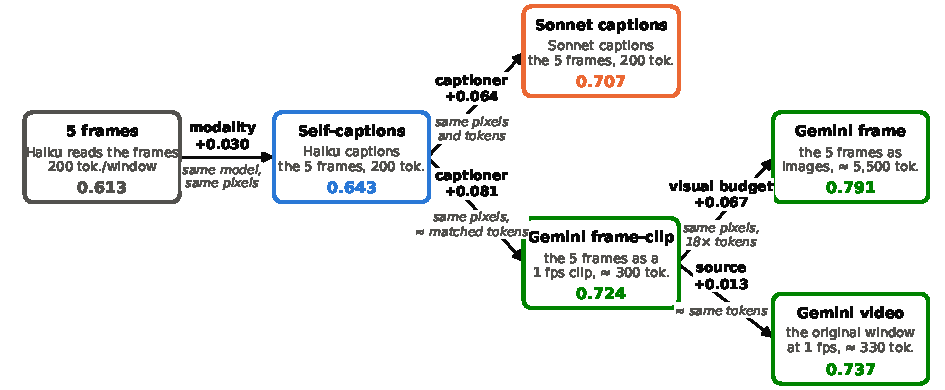
\includegraphics[width=\textwidth]{caption_index_fig0_design.pdf}
\caption{The design. Haiku reads every box (accuracy on the 297 confirmatory questions); the colour marks the captioner. Each arrow changes one thing, and its label is the effect, the accuracy difference between its two boxes, with what the arrow holds fixed below it. The effects add up along each path, e.g.\ Gemini frame − 5 frames = modality + captioner + visual budget. CIs are in Table~\ref{tab:effects}.}
\label{fig:design}
\end{figure*}

\textbf{The four effects.}\label{sec:effects} Each effect compares two arms that differ in one thing, with Haiku reading (Figure~\ref{fig:design}); the results with CIs are in Table~\ref{tab:effects} (\S\ref{sec:captioner}). \emph{Source}: Gemini's captions of the video window against its captions of the reader's frames played as a 1\,fps clip. Gemini samples the video at 1\,fps too, at the same instants, so the source effect measures what the original file adds at those instants (mostly resolution), not motion between them. \emph{Visual budget}: one captioner's captions of the same frames at two visual-token counts. \emph{Captioner}: two captioners' captions of the same frames at equal or matched visual tokens. \emph{Modality}: the reader on its self-captions against the reader on those frames (the two prompts also differ in the sentence that says what the evidence is; Appendix~\ref{app:prompts}). In the Claude chain, source and visual budget are zero by design. In the Gemini chain both branch from the frame-clip captions, so the terms add up along two paths: video captions − frames = source + captioner + modality, and frame captions − frames = visual budget + captioner + modality.

\textbf{Proposition~2 (break-even).} An index $\tau$ that costs $C(\tau)$ per video and $c_\tau$ per question pays for itself, against frames at $c_f$ per question, after
\[ \qbe = \frac{C(\tau)}{c_f - c_\tau} \]
questions per video, the break-even quantity. With a reader downgrade, $c_\tau$ is the cheaper reader's cost. If each of $W$ windows is captioned in its own call at cost $k$, and costs the reader $s_f$ as frames and $s_\tau$ as text, then $\qbe \to k / (s_f - s_\tau)$ as $W$ grows: on long videos the per-window prices set the break-even, not the fixed prompt.

\textbf{Omission.} If the same model answers correctly from the frames with the question in view, but its question-blind captions do not decide the question, the captioner could see the fact and did not write it down: the loss is an omission. Whether text could carry the fact needs a question-aware caption read without the frames, which we did not run.

\textbf{Retention}, (captions − question only) / (frames − question only), is the share of the frames' gain over the question alone that an index keeps.

\section{Results}
\label{sec:results}

\begin{table*}[t]
\centering
\footnotesize
\resizebox{\textwidth}{!}{\begin{tabular}{@{}llll@{}}
\toprule
Effect & Arms compared & Claude chain & Gemini chain \\
\midrule
Source & video captions − frame-clip captions & 0 by design & +0.013 [−0.030, +0.061] \\
Visual budget & frame captions − frame-clip captions & 0 by design (+0.003 at 448\,px) & +0.067 [+0.030, +0.108] \\
Captioner & other captioner − self-captions, same pixels & +0.064 [+0.017, +0.111] & +0.081 [+0.030, +0.131] \\
Modality & self-captions − 5 frames & +0.030 [−0.034, +0.094] & (same) \\
\midrule
\textit{Total} & captions − 5 frames & +0.094 [+0.044, +0.148] & video: +0.125; frame: +0.178 \\
\bottomrule
\end{tabular}}
\caption{The four effects, with Haiku reading. Accuracy differences on 297 questions, 95\% paired bootstrap CIs (the pre-registered P2 and P3: 98.33\%). In the Gemini chain, source and visual budget both branch from the frame-clip captions, so its terms add up along two paths (\S\ref{sec:theory}): video captions − frames = source + captioner + modality, and frame captions − frames = visual budget + captioner + modality.}
\label{tab:effects}
\end{table*}

All results are on the 297 confirmatory questions, and no question is missing from any arm. Differences are in accuracy, so +0.064 is 6.4 points.

Table~\ref{tab:main} lists the main arms (the variants are in Table~\ref{tab:variants}). Two rows anchor the rest. With the question and options alone, both readers score 0.41 (Haiku 0.411, Sonnet 0.414; difference +0.003 [−0.061, +0.064]), well above chance (≈ 0.30): the wording carries a strong prior, and the two readers share it. Given five frames per window, Sonnet scores 0.185 more than Haiku (0.798 vs.\ 0.613). Since the floor is shared, that whole gap comes from reading the input. Every index Haiku reads lands between these two points (0.643--0.791), and every index Sonnet reads lands below its frames (0.710--0.791).

\begin{table}[t]
\centering
\footnotesize
\setlength{\tabcolsep}{2.5pt}
\begin{tabular}{@{}lrrrr@{}}
\toprule
Reader, input & Acc. & In tok. & \$/q & Index \\
\midrule
H, question only & 0.411 & 1,025 & 1.09 & — \\
H, 5 frames & 0.613 & 1,520 & 2.04 & — \\
H, self-captions & 0.643 & 1,283 & 1.89 & 0.58 \\
H, Sonnet capt. & 0.707 & 1,280 & 1.81 & 9.10 \\
H, Gem.\ frame-clip & 0.724 & 1,232 & 1.67 & 7.60 \\
H, Gem.\ frame & 0.791 & 1,229 & 1.67 & 14.61 \\
H, Gem.\ video & 0.737 & 1,236 & 1.68 & 7.26 \\
\midrule
S, question only & 0.414 & 1,027 & 21.82 & — \\
S, 5 frames & 0.798 & 1,522 & 41.12 & — \\
S, Sonnet capt. & 0.710 & 1,282 & 30.89 & 9.10 \\
S, Gem.\ video & 0.791 & 1,238 & 28.68 & 7.26 \\
\midrule
Q, question only & 0.397 & 121 & — & — \\
Q, 5 frames & 0.657 & 529 & — & — \\
Q, Qwen capt. & 0.535 & 268 & — & — \\
Q, Sonnet capt. & 0.660 & 295 & — & 9.10 \\
Q, Gem.\ video & 0.697 & 264 & — & 7.26 \\
\bottomrule
\end{tabular}
\caption{Accuracy and list-price cost per question (297 questions; H = Haiku, S = Sonnet, Q = Qwen reading). Qwen runs on a free GPU, so it has no price; its input tokens have no CLI system prompt. Input tokens are the median per question and include the fixed reader prompt (≈ 1,025 tokens). \$/q is list-price dollars per question ×$10^{4}$, including output and thinking tokens. Index is the one-time captioning cost in dollars per video ×$10^{3}$, averaged over videos (\S\ref{sec:cost}). The variant arms are in Table~\ref{tab:variants}.}
\label{tab:main}
\end{table}

\subsection{Who writes the caption matters}
\label{sec:captioner}

Table~\ref{tab:effects} splits the caption effect into source, visual budget, captioner and modality effects. The pre-registered test is P3. With Haiku as the reader, Gemini's captions of exactly the reader's frames beat Haiku's self-captions by +0.148 [+0.088, +0.209], 2.5× the predicted +0.06. The gain is positive in every aspect (+0.10 to +0.20) and in every video type (Appendix~\ref{app:tables}).

P3 compares two captioners that spent different visual tokens on the same pixels. Gemini's image path encodes each 224\,px frame at ≈ 1,100 tokens, ≈ 5,500 per window, against Haiku's 200. Captioning the same frames as a 1\,fps clip through Gemini's video path (≈ 280--330 tokens per window, equal to the video arm's in 693 of 761 windows) splits P3 into two halves: a captioner effect at about matched visual tokens, +0.081 [+0.030, +0.131], \cl{} [+0.035, +0.125]; and a visual budget effect, +0.067 [+0.030, +0.108].

The source effect is near zero (+0.013 [−0.030, +0.061]): with captioner and visual tokens fixed, captions of the original video window are no more useful than captions of the reader's 224\,px frames. Gemini samples the window at the same 1\,fps instants and reduces each frame to ≈ 66 tokens, so little of the original file's resolution reaches the captioner, and nothing between the instants does. All four predictions for this split were within 0.02 of the results.

Within one model family, the match is exact. Sonnet captions the same five JPEGs per window, with the same prompt and effort as Haiku's self-captions, and its caption calls took exactly 2 more input tokens than Haiku's in every window (876). Only the captioning model differs. Haiku reads Sonnet's captions more accurately than its self-captions: \textbf{+0.064 [+0.017, +0.111]}, \cl{} [+0.011, +0.119]. The predicted +0.09 lies inside the CI. At about equal visual tokens, the two families' captioners are equally useful to Haiku (Sonnet − Gemini frame-clip captions, −0.017 [−0.071, +0.037]). On minimal pairs (\S\ref{sec:types}), where a guess cannot score, the captioner effect is +0.104 [+0.017, +0.190] in pair accuracy. On 738 further TempCompass questions about the same videos (\S\ref{sec:decide}), it is +0.072, \cl{} [+0.027, +0.119], and Gemini's video captions beat Haiku's self-captions by +0.122, \cl{} [+0.068, +0.177] (computed after that run, not predicted). With an open-weights reader the effect is larger: Qwen reads Sonnet's captions of the same frames +0.125 [+0.074, +0.175], \cl{} [+0.070, +0.182], more accurately than its self-captions (\S\ref{sec:robust}).

Unlike Gemini's, Claude's captioner gains nothing from a larger visual budget in the range we tested: Sonnet's captions of 448\,px frames, at 3.6× the visual tokens, are no more useful to Haiku, +0.003 [−0.037, +0.047] (Appendix~\ref{app:extra}).

\subsection{Text itself is not easier for the reader}
\label{sec:modality}

The modality effect asks whether a reader does better on its own words than on the pixels they came from. For Haiku this is the pre-registered P2: self-captions − 5 frames = +0.030 [−0.034, +0.094]. Both the prediction (−0.08) and any gain above +0.09 lie outside the CI. On 738 further questions about the same videos it is −0.064, \cl{} [−0.114, −0.014] (predicted +0.03; \S\ref{sec:decide}): Haiku's frames score higher on those questions, mostly on direction, so the sign for Haiku depends on the questions, but neither set shows a gain from its own words. IsoBench IsoBench \citep{isobench}, by contrast, finds 15--29 points for exact text renderings of images. For Sonnet, its self-captions cost accuracy: −0.088 [−0.135, −0.044], \cl{} [−0.140, −0.036], and −0.067 [−0.114, −0.024] when it captions the 448\,px frames. For Qwen, its self-captions cost −0.121 [−0.172, −0.071], \cl{} [−0.170, −0.074]; Qwen reads frames better than Haiku (0.657 vs.\ 0.613), and its captions are the least useful in the study (\S\ref{sec:robust}). So the modality effect is near 0 for the reader that reads frames worst (Haiku) and negative for the two that read them better.

\begin{figure}[t]
\centering
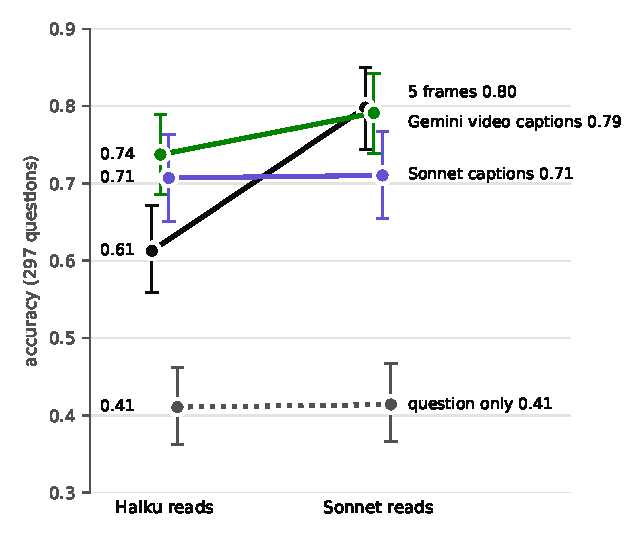
\includegraphics[width=\columnwidth]{caption_index_fig3_readers.pdf}
\caption{Accuracy by reader, in order of accuracy on frames, for the question alone, 5 frames, and the two indexes every reader read. 95\% CIs over clip clusters. The frames line crosses both index lines; Sonnet's captions are flat from Haiku to Sonnet, Gemini's are not.}
\label{fig:readers}
\end{figure}

Figure~\ref{fig:readers} shows why. From Haiku to Sonnet, accuracy on frames rises from 0.613 to 0.798, while accuracy on Sonnet's captions stays flat (0.707 → 0.710; Sonnet − Haiku +0.003 [−0.040, +0.047]). On these captions, a reader that costs 17× less per question loses nothing measurable. The tie holds on all four indexes Sonnet wrote (Sonnet − Haiku +0.000 to +0.020, every CI includes 0; Appendix~\ref{app:extra}): Haiku on frames is below what the captions hold and gains from them, and Sonnet is above it and loses. A Sonnet-written index is also Sonnet's own wording, so we cannot tell whether the tie comes from the index or from Sonnet reading its own words. The tie does not hold for every index. On Gemini's video captions Sonnet reads more than Haiku, +0.054 [+0.017, +0.091], and keeps 0.98, \cl{} [0.85, 1.13], of its frames' gain over the question alone, against 0.77, \cl{} [0.64, 0.90], on its self-captions (retention, \S\ref{sec:theory}). Qwen trails Haiku on every shared index (−0.04 to −0.08; the CI excludes 0 only on Gemini frame captions), almost all of it on two-clip videos. None of this was predicted, and it is exploratory. Haiku's advantage on captions does not come from starving the frames: captions still beat 448\,px frames at 1.76× the input tokens (Appendix~\ref{app:extra}).

\subsection{Where captions lose: video types and minimal pairs}
\label{sec:types}

Built videos (reversed, stacked, two-clip) are 54\% of the confirmatory set, and every stacked question is about speed and every two-clip question about order, so we report by type (Figure~\ref{fig:types}). On plain videos, the five arms lie within 0.09 of each other (0.80--0.89). They separate on the built videos.

\begin{figure}[t]
\centering
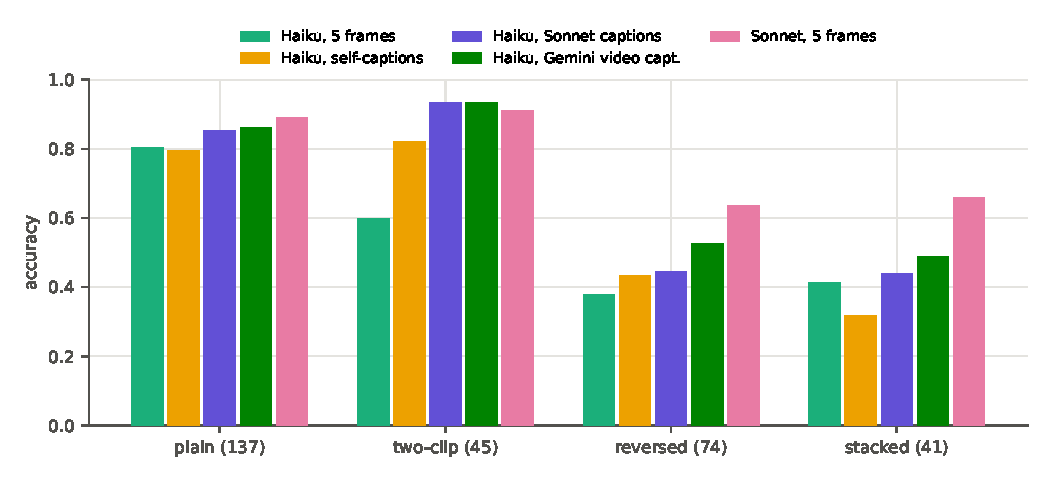
\includegraphics[width=\columnwidth]{caption_index_fig2_types.pdf}
\caption{Accuracy by video type for five arms (297 questions; n per type in brackets).}
\label{fig:types}
\end{figure}

Accuracy on one video cannot tell a representation that lost the fact from a reader that guessed. Minimal pairs can. Each of 193 confirmatory questions is asked again, with the same wording and option order, on a sibling video built from the same filmed clip whose correct option differs: the plain and the reversed version of a clip (107 pairs); another stacked version at other speeds (41); another arrangement of the same two clips (45). An arm that does not receive the fact gives the same answer on both videos, and gets at most one of them right. Table~\ref{tab:pairs} reports pair accuracy, the share of pairs answered correctly on both sides (chance 0.093), and the same-answer rate.

\begin{table}[t]
\centering
\footnotesize
\setlength{\tabcolsep}{3pt}
\begin{tabular}{@{}lrrrrr@{}}
\toprule
Arm & All & Rev. & Stack. & 2-clip & Same \\
 & & (107) & (41) & (45) & ans. \\
\midrule
H, 5 frames & 0.233 & 0.28 & 0.17 & 0.18 & 0.54 \\
H, self-captions & 0.326 & 0.33 & 0.10 & 0.53 & 0.42 \\
H, Sonnet capt. & 0.430 & 0.38 & 0.17 & 0.78 & 0.43 \\
H, Gem.\ video & 0.482 & 0.47 & 0.20 & 0.78 & 0.37 \\
S, 5 frames & 0.606 & 0.56 & 0.51 & 0.80 & 0.28 \\
S, Sonnet capt. & 0.430 & 0.40 & 0.10 & 0.80 & 0.39 \\
\bottomrule
\end{tabular}
\caption{Minimal pairs: pair accuracy by group, and the share of pairs with the same answer on both videos. Chance pair accuracy is 0.093.}
\label{tab:pairs}
\end{table}

\paragraph{Two-clip: captions help a weak reader.} From frames, Haiku must keep about ten small frames from two clips apart, and on two-clip pairs it is near chance (0.18). Its self-captions raise pair accuracy to 0.53, a modality effect of +0.36 [+0.16, +0.56] (+0.22 [+0.10, +0.35] \cl{} in accuracy), and Sonnet's captions raise its accuracy over its frames by +0.33, \cl{} [+0.20, +0.48]. Both were predicted. Describing each window before answering, in the same call, gains only +0.09 [−0.06, +0.24] here.

\paragraph{Stacked: question-blind captions drop the comparison.} Sonnet on frames answers 0.51 of stacked pairs correctly on both sides. Every caption arm scores 0.10--0.20, near pair chance, including Sonnet on its self-captions (0.10; −0.41 [−0.62, −0.23] against its frames). The captions do not say how the copies differ: they give the same answer on both videos of a pair more often than Sonnet on frames (Haiku on Sonnet captions +0.32 [+0.07, +0.55]). For a man jumping rope in two copies (answer: the one above is faster), Gemini writes ``An athletic man \ldots{} jumps rope in a split-screen video''. Sonnet sees the difference when it looks with the question in view, and loses it when it writes without the question. The loss lies in what a question-blind captioner writes, not in what it can see.

\paragraph{Reversed: captions narrate forward, or do not commit.} The question alone points to the forward event: both readers score below chance on reversed videos (Haiku 0.16, Sonnet 0.18). Sonnet on frames recovers part of the reversal (0.64), but its question-blind captions keep little of it (Sonnet on its self-captions −0.18, Haiku on them −0.19 against Sonnet on frames; Table~\ref{tab:bytype}). Sonnet's captions report reversals no more often than Haiku's (+0.01 [−0.08, +0.10]; a gain was predicted), and Gemini's a little more (+0.14 [+0.04, +0.24]). A reader that misses the reversal falls back to the prior: 0.59 (frames) and 0.65 (self-captions) of Sonnet's wrong answers on reversed videos equal its question-only answer, against 0.43 if errors were uniform. For a pile of salt played backwards (answer: shrinking), all five of Gemini's video captions describe salt pouring onto the pile.

\paragraph{Seen when asked, lost when written blind.} A low score might only mean that the built videos fooled the captioner. The arms separate the two causes, since the same model also reads the same pixels with the question in view. Table~\ref{tab:headroom} (descriptive) splits Sonnet's headroom into a perception shortfall, 1 − frames, and the modality effect, self-captions − frames: what Sonnet sees when asked but does not write down blind. On plain and two-clip videos the modality effect is ≈ 0, and the captions keep 0.95--1.00 of the frames' gain. On reversed videos Sonnet is misled even with the question in view (shortfall 0.36), and writing blind loses another 0.18. On stacked videos it sees the comparison when asked (0.66), but its blind captions keep little of it (retention 0.21, wide CI). For Haiku reading Sonnet's captions, captions − frames is positive on every type (Appendix~\ref{app:extra}).

\subsection{Why caption arms fail: an audit}
\label{sec:audit}

For every caption set and question that a reader got wrong in one of seven reader arms (442 items; two readers share some caption sets), a judge (Sonnet) saw the captions, question, options and correct answer, and labelled the captions as stating the correct option (a reader error), a wrong option (a misstatement), or neither (an omission), quoting the caption as evidence (Appendix~\ref{app:prompts}; Table~\ref{tab:audit}).

Omission dominates: 0.61--0.73 of every arm's wrong answers come from captions that do not decide the question. Misstatements are 0.15--0.28, and reader errors only 0.05--0.17, below the predicted 0.15--0.25. A fact missing from the index cannot be read from it by any reader, which fits the readers' tie on Sonnet's captions (\S\ref{sec:modality}). As predicted, 0.93--1.00 of stacked failures are omissions in every arm (predicted ≥ 0.70). On reversed videos, misstatement (forward narration) is only 0.28--0.45 (predicted ≥ 0.50) and omission 0.45--0.62: captions narrate the forward event or do not commit to a direction. The judge also wrote one of the caption sets it labels. One author's 40 labels, stratified by the judge's label and blind to it, agree at κ = 0.81 [0.64, 0.96] (threshold 0.6, set in advance); all 5 disagreements are items the author left ``silent'', so if anything Table~\ref{tab:audit} undercounts omission.

\begin{table}[t]
\centering
\footnotesize
\setlength{\tabcolsep}{3pt}
\begin{tabular}{@{}lrrrr@{}}
\toprule
Reader arm & Reader err. & Misstat. & Omission & n \\
\midrule
H, self-captions & 0.08 & 0.28 & 0.63 & 106 \\
H, Sonnet capt. & 0.13 & 0.26 & 0.61 & 87 \\
H, Gem.\ frame-clip & 0.17 & 0.15 & 0.68 & 82 \\
H, Gem.\ frame & 0.10 & 0.18 & 0.73 & 62 \\
H, Gem.\ video & 0.10 & 0.21 & 0.69 & 78 \\
S, Gem.\ video & 0.05 & 0.24 & 0.71 & 62 \\
S, Sonnet capt. & 0.08 & 0.26 & 0.66 & 86 \\
\bottomrule
\end{tabular}
\caption{Caption audit: share of each reader arm's wrong answers by the judge's label of the captions. Reader error = the captions state the correct option; misstatement = a wrong option; omission = neither. n = wrong answers.}
\label{tab:audit}
\end{table}

\subsection{From question-blind to question-aware}
\label{sec:aware}

Two arms move the captioner toward the question. Neither changes the confirmatory captioner prompt.

\paragraph{Describe, then answer.} Haiku sees the 5 frames per window and the question, writes one sentence per window, and then answers, all in one call. It scores 0.684, +0.071 over the frames arm, \cl{} [+0.029, +0.114] (predicted +0.03). The gain is on reversed and stacked videos (+0.12 each). On stacked videos, this question-aware description beats the question-blind self-captions by \textbf{+0.22 [+0.09, +0.37]}. This fits an omission (\S\ref{sec:theory}): with the question in view, Haiku catches what its blind captions leave out. Because the arm still has the frames when it answers, it does not show that text alone could carry the comparison. This arm is not an index: it reads the frames at every question, and it costs 2× the frames arm per question (\$0.000415 vs.\ \$0.000204), mostly in thinking tokens.

\paragraph{Telling the captioner the kinds of question.} One added prompt bullet that names the five kinds of question to come (Appendix~\ref{app:prompts}) gives a task-aware index. Over Sonnet's whole-video captions it gains +0.040 [+0.003, +0.081] with Sonnet reading and +0.027 [−0.013, +0.067] with Haiku (both predicted +0.03), but nothing on stacked videos (Appendix~\ref{app:extra}).

\subsection{When to read the index: a decision rule}
\label{sec:decide}

A system that keeps both the index and the frames could choose per question. Where a reader's answers from the two disagree, on 20\% of questions, either can be right: Haiku's self-captions win 34 such questions and lose 25, Qwen on Sonnet's captions 26 and 25. We asked, in three logged steps, whether anything known before the question is read says which (Appendix~\ref{app:decide}).

\paragraph{Scores of the video and its captions do not predict.} Two question-blind scores were tested first, as predictors of a \emph{loss} (a reader right on its frames and wrong on its self-captions) within each video type: \emph{motion}, the mean SigLIP~2 \citep{siglip2} distance between consecutive frames, and \emph{coverage}, the SigLIP~2 similarity of each caption to its window's frames. Both fail: stratified AUC 0.42 [0.28, 0.57] for motion (predicted 0.60; the point estimate is on the wrong side) and 0.53 [0.38, 0.67] for coverage (predicted 0.58; 97.5\% CIs over clip clusters). They recover the construction instead (two-clip videos move most and lose least) and add nothing to the video type. A development run then fit logistic models to the 898 disagreements of 15 reader--index pairs. The question's aspect and the pair (reader, captioner family) give an out-of-fold AUC of 0.756 [0.705, 0.803]. Adding motion, cuts, the number of windows, coverage, or how often the captions use the aspect's words (``faster'', ``leftward'', ``then'') changes it by −0.002 to +0.002, and a selection rule fixed in advance chose aspect + pair. The AUC comes mostly from the pair. Against the best fixed choice per pair, the rule gains +0.005 [−0.003, +0.014] in accuracy, and its one signal within a pair is that speed questions favour the frames.

\paragraph{The frozen rule on new questions.} We froze the rule and tested it on the 738 TempCompass questions about the confirmatory videos that the confirmatory set does not ask (2,952 Haiku calls on frames, self-captions, Sonnet captions and Gemini video captions). In words, the rule says: read Gemini's captions; with Claude's captions, read the frames on speed questions. On the 492 disagreements its AUC is \textbf{0.666} [0.587, 0.743] (97.5\%, \cl; predicted 0.68). The speed shift, P(index right | speed) − P(index right | other aspects) on disagreements, is −0.148 [−0.320, +0.007] (0.39 against 0.54; predicted −0.25), so the second primary test narrowly fails, although the sign holds for all three indexes. The rule beats always reading the index by +0.013, \cl{} [+0.002, +0.026] (predicted ≈ 0), but not always reading the frames (+0.014 [−0.013, +0.041]). One shift was not predicted: Haiku's frames score 0.699 on these questions against 0.613 on the confirmatory ones, mostly on direction, where reworded questions about the same videos give 0.50 against 0.30. The index's value for a weak reader thus moves with how the questions are worded, by as much as the effects of \S\ref{sec:captioner}--\ref{sec:modality}. The test reuses the confirmatory videos, and on the 67 disagreements about an aspect the confirmatory set had not asked of the video, the rule does not hold (AUC 0.40, descriptive).

\subsection{Robustness checks and nulls}
\label{sec:robust}

\paragraph{An open-weights reader.} Qwen2.5-VL-7B-Instruct, with greedy decoding and the same prompts, reads eight arms and captions every window from exactly the 5 frames. Unparsed answers count as wrong (Appendix~\ref{app:extra}). Qwen reads frames well (0.657, above Haiku's 0.613), but its self-captions are the weakest in the study, even for itself (Haiku's are +0.067 [+0.020, +0.114] better). Besides the captioner and modality effects (\S\ref{sec:captioner}--\ref{sec:modality}; the modality cost of −0.121 was predicted as −0.01), Gemini's video captions add only +0.040 [−0.010, +0.091] over Qwen's frames (predicted +0.12).

\paragraph{Other checks (Appendix~\ref{app:extra}).} One Sonnet caption per video instead of one per window does no better (+0.013 with Haiku reading, +0.010 with Sonnet; predicted ≈ 0), at half the index cost. Re-captioning identical input changes 10--17\% of answers, so comparisons between caption arms, and by type, are noisy. The pre-registered aspect contrast (P1) did not pass: −0.101 [−0.231, +0.028] for Sonnet, half the predicted −0.20.

\begin{table}[t]
\centering
\footnotesize
\setlength{\tabcolsep}{2.5pt}
\resizebox{\columnwidth}{!}{\begin{tabular}{@{}lrrrrr@{}}
\toprule
Type (n) & Q.\ only & Frames & Self-capt. & Modality & Retention \\
\midrule
plain (137) & 0.61 & 0.89 & 0.88 & −0.01 [−0.06, +0.03] & 0.95 [0.79, 1.12] \\
two-clip (45) & 0.29 & 0.91 & 0.91 & +0.00 [−0.06, +0.07] & 1.00 [0.91, 1.12] \\
reversed (74) & 0.18 & 0.64 & 0.46 & \textbf{−0.18} [−0.30, −0.05] & 0.62 [0.35, 0.88] \\
stacked (41) & 0.32 & 0.66 & 0.39 & \textbf{−0.27} [−0.47, −0.09] & 0.21 [−0.27, 0.67] \\
\midrule
all (297) & 0.41 & 0.80 & 0.71 & −0.09 [−0.14, −0.04] & 0.77 [0.64, 0.90] \\
\bottomrule
\end{tabular}}
\caption{Where Sonnet's headroom goes, by video type (Sonnet as captioner and reader; 95\% CIs over clip clusters). The perception shortfall is 1 − frames; modality = self-captions − frames.}
\label{tab:headroom}
\end{table}

\section{Cost and break-even}
\label{sec:cost}

\paragraph{Accounting.} We price every call at list price: Claude Haiku 5.5 at \$0.10 / \$0.50 and Sonnet 5.5 at \$2 / \$10 per million input / output tokens, with thinking billed as output (this equals the CLI's reported cost on every call), and Gemini captioning at \$0.50 / \$3.00. A reader's cost per question, $c$, is the mean over the 297 questions, and an index's cost per video, $C(\tau)$, is the cost of captioning all its windows once. \qbe{} follows Proposition~2; its CIs resample questions, and so videos, since each video has one question.

\begin{figure*}[t]
\centering
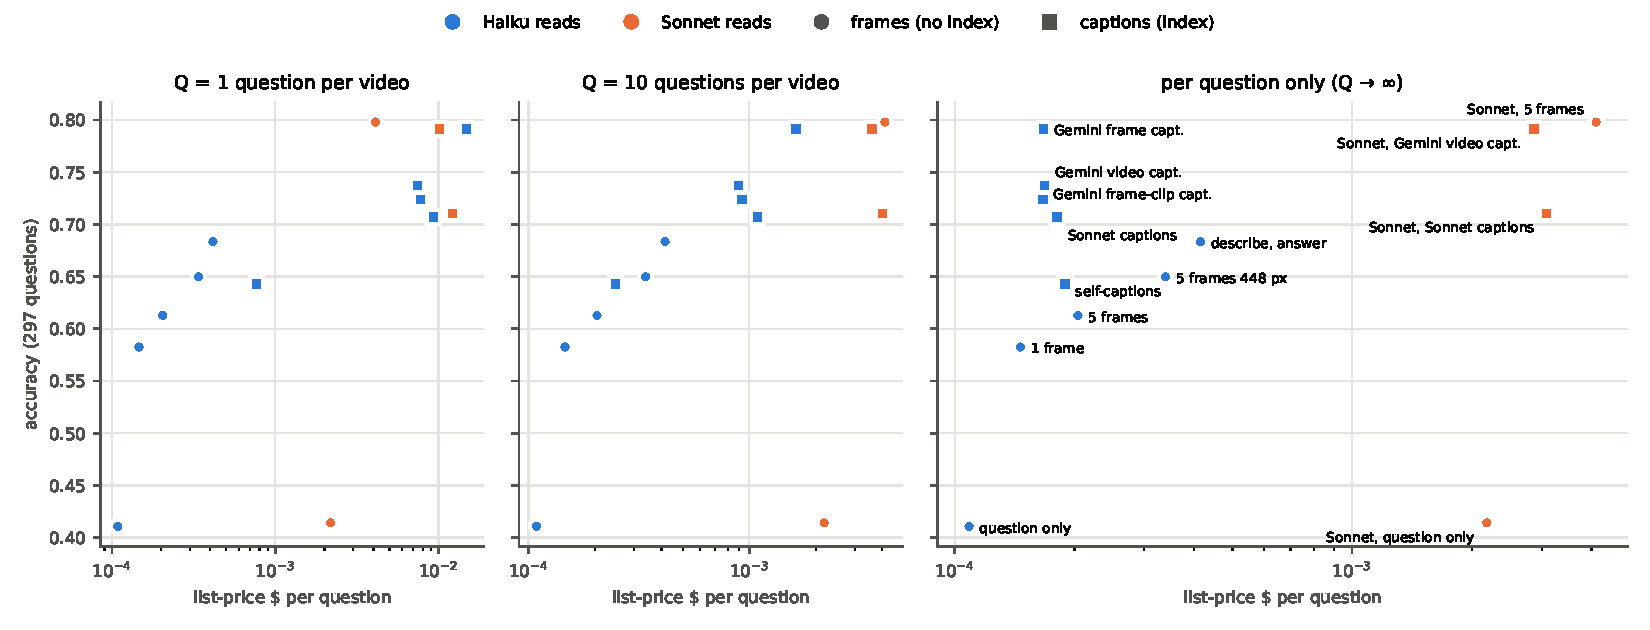
\includegraphics[width=\textwidth]{caption_index_fig1_cost.pdf}
\caption{Accuracy against list-price \$ per question (log scale), one point per arm, with the index cost spread over Q = 1, 10 and infinitely many questions per video. Circles are frame arms, and squares are index arms. Question only (0.41 for both readers) is below the axis; the 448\,px caption, whole-video and aspect-aware variants are in Table~\ref{tab:variants} only.}
\label{fig:cost}
\end{figure*}

\paragraph{For one reader, the index saves little.} Against 5 frames, Gemini video captions save 18\% per question for Haiku and 30\% for Sonnet. The percentages are small because the fixed reader prompt (≈ 1,025 tokens) dominates the input: captions cut the video-content tokens to 43\% of the frames', but the input tokens only to 81\%. The break-even depends on the absolute saving instead, which is small for a cheap reader: Sonnet on Gemini video captions repays after $\qbe = 5.8$ [5.2, 6.5], at equal accuracy (−0.007 [−0.054, +0.040]), and Haiku only after 202 [156, 279], though 0.125 more accurate than on its frames.

\paragraph{The reader downgrade is what pays.} Per question, Haiku on any index written by a stronger captioner costs 1/23 to 1/26 of Sonnet on frames (Table~\ref{tab:main}), and the index repays its captioning within 1.2--3.7 questions per video: 1.2--1.3 for the whole-video indexes, 1.8--3.7 for the per-window ones (Table~\ref{tab:qbe} in Appendix~\ref{app:extra}). At 10 questions per video (Figure~\ref{fig:cost}, middle), every index Haiku reads costs less than half of Sonnet on frames, captioning included. The accuracy cost of the downgrade depends on the index. Gemini frame captions let Haiku match Sonnet on frames (−0.007 [−0.057, +0.044]), but they are the most expensive index (\$0.0146 per video), because Gemini's image path spends ≈ 5,500 visual tokens per window. In the Claude chain, where Sonnet captions once and Haiku answers, the cost is −0.091 [−0.145, −0.040] at $\qbe = 2.3$; aspect-aware captions bring it to −0.051 [−0.104, +0.000] at $\qbe = 1.3$.

\paragraph{Without the CLI's prompt.} The CLI adds ≈ 850 input tokens to every Claude call, which an API deployment would drop or cache. Without them, the reader downgrade costs 1/25 to 1/34 of Sonnet on frames per question and repays within 1.4--6.3 questions per video (Appendix~\ref{app:extra}).

\paragraph{Longer videos.} Projected by Proposition~2 to videos whose every window is read (Appendix~\ref{app:extra}), captions save more per question as videos grow, but \qbe{} does not fall, because captioning grows with every window too: for the reader downgrade it rises from 1.8--3.7 to 4.5--8.9 at one minute.

\section{Related work}
\label{sec:related}
\textbf{Caption, then reason.} Composing models through language goes back to Socratic Models \citep{socratic}. Many video QA systems caption first and reason over the text \citep{llovi,videotree,silvr,vamos}, or let an LLM agent choose which frames to caption \citep{videoagent}; LLoVi already finds that the captioner matters. Caption indexes and memories reuse the captions across questions \citep{cfd,capmem,sprout,vidctx}. Caption utility is also judged by QA rather than by similarity \citep{captionqa,capquiz,visil}, and CapRL \citep{caprl} trains a captioner on it. Prism \citep{prism} and MetaCaptioner \citep{metacaptioner} vary the captioner in front of a fixed reader. CapMem \citep{capmem} is closest: on long egocentric video, Qwen readers read six Qwen captioners' captions of the same frames, and their own, but it does not split source from visual budget, cross families or price a cheaper reader. Its stronger reader gains on fixed captions; on Sonnet's captions we find no such gain, and on Gemini's a small one.

\textbf{Text or pixels.} IsoBench \citep{isobench} finds 15--29 points for exact text renderings of images, and TokenSwap \citep{tokenswap} studies the same contrast. For a model reading its own description, the sign varies: own captions give a weak 7B model +22 to +29 points on synthetic image tasks \citep{captionthis}, while appending the model's own caption costs about 10 points on HallusionBench \citep{geass}, and a one-call ``state first'' prompt does not help on charts \citep{seeingsolving}. Our modality effect (at most +0.09 for Haiku, negative for Sonnet and Qwen) fits CapMem's sign on videos under 20 minutes.

\textbf{Temporal video and cost.} Minimal pairs follow TempCompass's conflicting videos \citep{tempcompass}, MotionBlind \citep{motionblind} and TimeBlind \citep{timeblind}; we apply them to representations rather than to models. Video models often fail direction, speed and reversal from pixels too \citep{whichway,arrowoftime,reversaldrop,t3}, which fits P1's null. Cascades and routers send each query to a cheaper model when they can \citep{frugalgpt,routellm,safecascade}; an index makes the cheap route possible for video. We found no paper that solves for break-even with a reader downgrade; on cost see also \citet{mit3,remembr,lohi,vei,agentsmatter}.

\section{Discussion}
\label{sec:discussion}
\textbf{Using an index.} Four rules follow from the arms. First, caption with a stronger model than the reader: self-captions gain a reader at most 0.09, and cost Sonnet and Qwen 0.09--0.12. Second, the saving is in the reader downgrade, not in the modality: the same reader saves 18--30\% per question, a cheaper reader 23--26×, repaid within a few questions per video. Third, keep the frames for questions that compare copies or ask direction: there a blind index loses what the captioner did not write, and naming the kinds of question to the captioner recovers little (\S\ref{sec:aware}). Fourth, to choose per question between a kept index and the frames, the question's aspect and the reader and captioner are what we found to predict which is right (\S\ref{sec:decide}). Scores of the video's motion or of the captions' coverage did not, so a rule of the form ``this video scores $y$, so captions suit it'' is not supported on these videos.

\textbf{Why the baselines are needed.} The same captions help Haiku and cost Sonnet (retention 1.47, 0.77): without self-caption, frames and question-only arms, a ``caption effect'' mixes captioner, modality and prior.

\textbf{Future work.} Videos released after the readers' training data, with answers made by editing them, would rule out contamination. Asking which candidate fills a masked span compares the modalities on reconstruction: frame continuity wins over 1\,s gaps (Appendix~\ref{app:extra}), but the missing twenty minutes of a wedding (vows, rings) are easier to guess from script knowledge than from pixels. Long videos would test where captioning everything stops paying.

\section{Conclusion}
Given exactly the reader's frames, a stronger captioner's question-blind captions make Claude Haiku and an open 7B reader more accurate, while no reader gains more than 0.09 from its self-captions. The index pays through the cheaper reader, which on Sonnet's captions reads as well as Sonnet does. It loses what a captioner does not write without the question: comparisons between two copies of a clip, and reversals. Which of the index and the frames to trust on a question is predicted by the question's aspect and the models, not by scores of the video or its captions.

\section*{Limitations}
\textbf{Scope.} We test one benchmark, short clips (median 9.7\,s) and multiple-choice questions. 54\% of the confirmatory videos are manipulated (reversed, stacked, two-clip), so overall accuracies mix natural video with stress tests; plain videos are reported separately (Table~\ref{tab:headroom}). The costs for longer videos (\S\ref{sec:cost}) are projections from short clips, for a reader that reads every window. All captions follow one generic, question-blind prompt that does not mention the benchmark's manipulations; captions written for retrieval or question answering may keep more.

\textbf{Contamination.} TempCompass (March 2024) predates every reader's training data (June 2026 for the Claude models), so the readers may have seen its questions. The question alone scores 0.40--0.41, 0.11 above chance, but this comes from a third of the questions. For 197 of the 297 confirmatory questions, TempCompass itself asks the same question, with the same options, of another video with another answer, so a remembered answer cannot fit both. On these 197 the question alone is at chance (Haiku +0.02, Sonnet $-$0.01), and the headline effects keep their signs: captioner +0.08 [+0.02, +0.14], the readers' tie on Sonnet's captions (Haiku − Sonnet) +0.02 [$-$0.04, +0.07], Haiku on Sonnet's captions vs.\ Sonnet on frames $-$0.11 [$-$0.18, $-$0.04]. None is smaller there than on the other 100. On minimal-pair accuracy, which a text-only answer cannot earn, they hold too (Table~\ref{tab:pairs}; the tie is 0.00 [$-$0.07, +0.06]). We did not extend the study to EgoSchema \citep{egoschema}, because in a development run Sonnet scored 0.72 from the question alone (chance 0.20; 39 questions).

\textbf{Readers.} The closed readers run through a CLI, so its system prompt is part of every input and temperature is not controlled. Costs are at list price for these calls; \S\ref{sec:cost} also reports them without the CLI's prompt. Thinking is decided per call by the model (effort medium), so it is observed, not controlled. Mitigations are pinned model IDs, isolation checked on every call, released outputs, and an open-weights reader with greedy decoding that replicates the captioner and modality results (\S\ref{sec:robust}); it is one 7B model, with its own default system prompt. In the main chain Claude reads Claude's captions; the Gemini chain and the Qwen reader check this. Haiku's accuracy on frames dropped from the development to the confirmatory set (0.70 to 0.61); about half of the drop is the different mix of video types.

\textbf{Inference.} Questions share filmed clips, so we also report CIs over clip clusters. Most claims beyond the pre-registered test are exploratory: each follow-up was predicted in writing before it ran, but the readers' tie on Sonnet's captions, the thinking pattern and the analysis by video type of the first two runs were not. The audit's judge (Sonnet) also wrote one of the caption sets it judges; 40 blind hand labels check it (κ = 0.81). The decision rule (\S\ref{sec:decide}) was tested on new questions about the confirmatory videos, not on new videos; 618 of the 738 ask the same aspect of a video as a confirmatory question, mostly reworded, so the test is closer to a replication than to an independent sample. Rewording alone moved Haiku's accuracy on frames by 0.2 on direction questions, so accuracies for one reader depend on the question set as well as on the videos.

\textbf{Question-blind captions} drop what the question needs and the captioner did not write (stacked comparisons, reversals). Sonnet sees the stacked comparison on frames, and Haiku recovers part of it when it describes the frames with the question in view (\S\ref{sec:aware}), so the loss comes from writing blind. Whether a question-aware text index would keep it is untested: our question-aware arm still had the frames.

\section*{Ethics Statement}
The videos and questions are TempCompass's (CC BY-NC 4.0); we release the captions under the same licence and do not redistribute videos or frames. No human subjects took part; one author labelled 40 audit items. \textbf{Compute.} The TempCompass study made about 22,150 Claude calls (≈ \$22 at list price, run on a subscription), spent \$9.67 on Gemini captioning, and ran Qwen on a free Kaggle GPU \draftnote{GPU hours}. \textbf{AI assistance.} \draftnote{Author to confirm the wording.} Claude (through Claude Code) wrote analysis code, ran the experiments, and drafted and edited text under the author's direction; the author checked the reported numbers against the logged outputs and is responsible for the content.

\bibliography{caption_index}

\appendix

\section{Prompts}
\label{app:prompts}

All prompts are given exactly as sent. Text in braces is filled in per call.

\paragraph{Caption prompt.} Every captioner gets the same prompt. For frames (Haiku, Sonnet, and Gemini's frame and frame-clip captions), the first sentence is:
\begin{lstlisting}
The attached images are {n} frames from a {d}-second video clip, taken one second apart and shown in time order. Describe what happens in the clip, in one or two sentences of at most 45 words in total.
\end{lstlisting}
For Gemini's video captions, it is ``Describe what happens in the attached 5-second video clip, in one or two sentences of at most 45 words in total.'' The rest is the same for all:
\begin{lstlisting}
* Start with what happens: what the people, animals or machines do, or, if nothing in the clip acts, how the scene or the camera view changes.
* Then add the details that set this moment apart: the key objects and any on-screen text, but do not transcribe subtitles, clocks, timestamps, dates or numbering (such as day, part or step numbers), and leave out watermarks and channel logos.
* Describe the setting in a few words at most.
* Mention camera movement only when the camera clearly moves.
* Describe what is seen, not what is heard.
* Include enough details so someone who hasn't seen the video could understand what's happening.
* If a description cannot be generated, write "ERROR".
\end{lstlisting}
The whole-video captions (\S\ref{sec:robust}) get all of a video's frames in one call, and the length clause scales with the number of windows (for two windows: ``in at most 4 sentences of at most 90 words in total''). The aspect-aware captions (\S\ref{sec:aware}) add one bullet before the last:
\begin{lstlisting}
* The description will be used later to answer questions about the actions, the speed of the movements, the direction of the movements, the order of the events, and changes in the attributes of things (such as size, colour, shape or state). State these whenever the frames show them.
\end{lstlisting}

\paragraph{Reader prompt.}
\begin{lstlisting}
Answer a multiple-choice question about a video clip that is {duration} seconds long. There is no sound.

{modality}

{evidence}

Question: {stem}
{options}

Answer with JSON only, in this format: {"answer": "<letter>"}, with one of the letters {letters}.
\end{lstlisting}
The evidence is the frames or the captions, each window labelled with its time span (``0-5 s:''). The modality sentence is, for frames:
\begin{lstlisting}
The video was split into windows of 5 seconds (the last one may be shorter). Each window is shown as its frames taken one second apart, in time order.
\end{lstlisting}
for captions:
\begin{lstlisting}
The video was split into windows of 5 seconds (the last one may be shorter). Each window is given as a short description of what can be seen in it, in time order. Each description was written by an AI model that watched only that one window, without sound, and knew nothing about the rest of the video.
\end{lstlisting}
for whole-video captions:
\begin{lstlisting}
The video is given as a single description of what can be seen in it. The description was written by an AI model that watched the whole video, without sound.
\end{lstlisting}
for one frame per window, ``\ldots{} Each window is shown as one frame from its middle, in time order.''; and for the question only, ``You cannot see the video. Give your best guess from the question and options alone.''

\paragraph{Describe, then answer.} The reader prompt with frames, with the last paragraph replaced by:
\begin{lstlisting}
First describe each window in one sentence, in time order: what can be seen in it and what happens. Then answer. Answer with JSON only, in this format: {"windows": ["<window 1>", "<window 2>", ...], "answer": "<letter>"}, with one description per window and one of the letters {letters}.
\end{lstlisting}

\paragraph{Audit judge (\S\ref{sec:audit}).}
\begin{lstlisting}
You are checking whether written descriptions of a video contain the answer to a question about it.

The video is {duration} seconds long, without sound. It was split into windows of 5 seconds (the last one may be shorter). An AI model wrote one description per window, seeing only that one window and not the question:

{captions}

Question: {stem}
{options}

The correct answer is {answer}. {answer_text}

Judge the descriptions only, not what you think the video shows. Choose one label:
- "correct": the descriptions state the correct answer, or imply it clearly enough that a careful reader would choose it.
- "wrong": the descriptions state, or clearly imply, a different option.
- "silent": the descriptions do not decide between the options: the fact needed is missing or too vague.

Answer with JSON only, in this format: {"label": "<correct|wrong|silent>", "evidence": "<a short quote from the descriptions, or an empty string>"}
\end{lstlisting}

\section{Development phase and predictions}
\label{app:dev}

\paragraph{Development phase.} The hypotheses came from 100 development questions (20 per aspect, one per video, on videos the confirmatory set does not use), read by Haiku (question only, Gemini video captions, 1 and 5 frames per window) and Sonnet (Gemini video captions and 5 frames), and on 50 of them by Haiku with its self-captions. On them, Haiku on Gemini captions tied Haiku on 5 frames (+0.01 [−0.07, +0.09]); Sonnet lost on the captions (−0.07 [−0.15, 0.00]), mostly on direction and speed; and Haiku's self-captions were below its frames (−0.10 [−0.22, +0.02]) and below Gemini's captions (−0.08 [−0.18, 0.00]). These gave P1 (captions lose direction and speed: the grouping {direction, speed} against the other three aspects was fixed before any confirmatory call), P2 (no modality advantage, predicted −0.08) and P3 (the captioner adds usable information, +0.06). The development predictions were too pessimistic about captions: S1, S3, S5 and S6 all came out higher than predicted (Table~\ref{tab:preds}). Part of the shift is the mix of video types: built videos are 40\% of the development set and 54\% of the confirmatory set, and weighting the confirmatory accuracies by the development mix accounts for about half of Haiku's drop on frames (0.70 → 0.61).

\paragraph{Predictions against results.} Every exploratory term was written down with a predicted value and committed before its first call. Table~\ref{tab:preds} lists every predicted term. Of the 56 accuracy differences in it, the prediction lies inside the result's CI for 41, and for 39 of the 47 after C1. Of the 50 non-zero predictions, 47 have the sign of the result; the three exceptions are P2 and S2, both set from the 50 development questions, and A8's modality term. The median absolute difference between prediction and estimate is 0.024. The misses after C1 are C4e (Sonnet's pair-accuracy loss on its self-captions, larger than predicted), three open-reader terms (C12a, d, f), whose predictions treated Qwen as a weaker Haiku (it reads frames better than Haiku and writes less useful captions; \S\ref{sec:robust}), and four A8 terms, which all missed in the same direction: Haiku's frames were stronger on A8's questions than on the confirmatory ones (\S\ref{sec:decide}). Of the six AUC and speed-shift terms of A6 and A8, five have the prediction inside the CI (A6's gain over video type at its upper end); of the four primary tests among them, only A8's AUC passes.

\begin{table*}[t]
\centering
\scriptsize
\setlength{\tabcolsep}{3pt}
\resizebox{0.49\textwidth}{!}{\begin{tabular}[t]{@{}llr@{}}
\toprule
Term & Pred. & Result [95\% CI] \\
\midrule
\multicolumn{3}{@{}l}{\textit{C1, pre-registered; P1--P3 with 98.33\% CIs}} \\
P1 aspect contrast, S reads & −0.20 & −0.101 [−0.231, +0.028] \\
P2 modality, H & −0.08 & +0.030 [−0.034, +0.094] \\
P3 H: Gem.\ frame − self capt. & +0.06 & +0.148 [+0.088, +0.209] \\
S1 S: Gem.\ video capt. − frames & −0.07 & −0.007 [−0.054, +0.040] \\
S2 H: Gem.\ video − frame capt. & +0.02 & −0.054 [−0.098, −0.013] \\
S3 H: Gem.\ video capt. − frames & 0.00 & +0.125 [+0.071, +0.178] \\
S4 aspect contrast, H reads & −0.12 & −0.055 [−0.172, +0.060] \\
S5 H: Gem.\ video capt. − 1 frame & +0.05 & +0.155 [+0.098, +0.212] \\
S6 H on Gem.\ video − S on frames & −0.13 & −0.061 [−0.111, −0.010] \\
\multicolumn{3}{@{}l}{\textit{C2, frame-clip captions (H reads)}} \\
C2a frame-clip − self capt. & +0.10 & +0.081 [+0.030, +0.131] \\
C2b frame − frame-clip capt. & +0.05 & +0.067 [+0.030, +0.108] \\
C2c video − frame-clip capt. & 0.00 & +0.013 [−0.030, +0.061] \\
\multicolumn{3}{@{}l}{\textit{C3, Sonnet captions (H reads)}} \\
C3a Sonnet − self capt. & +0.09 & +0.064 [+0.017, +0.111] \\
C3b Sonnet capt. − frames & +0.12 & +0.094 [+0.044, +0.148] \\
C3c H on Sonnet capt. − S on frames & −0.07 & −0.091 [−0.145, −0.040] \\
C3d Sonnet − Gem.\ frame-clip capt. & 0.00 & −0.017 [−0.071, +0.037] \\
\multicolumn{3}{@{}l}{\textit{C4, minimal pairs (pair accuracy, \cl{} CIs)}} \\
C4a H: self capt. − frames & +0.06 & +0.093 [+0.028, +0.161] \\
C4b H: Sonnet − self capt. & +0.09 & +0.104 [+0.017, +0.190] \\
C4c H on Sonnet capt. − S on frames & −0.12 & −0.176 [−0.276, −0.079] \\
C4d H: Gem.\ video capt. − frames & +0.18 & +0.249 [+0.173, +0.319] \\
C4e S: own capt. − frames & −0.08 & −0.176 [−0.260, −0.093] \\
\multicolumn{3}{@{}l}{\textit{C5, describe, then answer (H, \cl{} CIs)}} \\
C5a describe − frames & +0.03 & +0.071 [+0.029, +0.114] \\
C5b describe − self capt. & 0.00 & +0.040 [−0.011, +0.092] \\
\multicolumn{3}{@{}l}{\textit{C6, 448\,px frames (H reads)}} \\
C6a 448 − 224\,px frames & +0.04 & +0.037 [−0.010, +0.084] \\
C6b Sonnet capt. − 448\,px frames & +0.07 & +0.057 [+0.003, +0.111] \\
C6c Gem.\ video capt. − 448\,px frames & +0.08 & +0.088 [+0.037, +0.138] \\
C6d Gem.\ frame capt. − 448\,px frames & +0.13 & +0.141 [+0.088, +0.195] \\
\multicolumn{3}{@{}l}{\textit{A8, frozen decision rule, 738 new questions (H, \cl{} CIs)}} \\
H1 rule's AUC (97.5\%) & 0.68 & 0.666 [0.587, 0.743] \\
H2 speed shift (97.5\%) & −0.25 & −0.148 [−0.320, +0.007] \\
self capt. − frames & +0.03 & −0.064 [−0.114, −0.014] \\
Sonnet capt. − frames & +0.09 & +0.008 [−0.026, +0.042] \\
Gem.\ video capt. − frames & +0.12 & +0.058 [+0.017, +0.098] \\
rule − always index & +0.005 & +0.013 [+0.002, +0.026] \\
rule − always frames & +0.08 & +0.014 [−0.013, +0.041] \\
speed only − always index & +0.005 & +0.013 [−0.002, +0.028] \\
\bottomrule
\end{tabular}}\hfill
\resizebox{0.49\textwidth}{!}{\begin{tabular}[t]{@{}llr@{}}
\toprule
Term & Pred. & Result [95\% CI] \\
\midrule
\multicolumn{3}{@{}l}{\textit{C7, audit: reader error / misstatement / omission}} \\
H, self capt. & .20 / .30 / .50 & .08 / .28 / .63 \\
H, Gem.\ video capt. & .25 / .30 / .45 & .10 / .21 / .69 \\
S, Gem.\ video capt. & .15 / .35 / .50 & .05 / .24 / .71 \\
stacked: omission & ≥ .70 & .93--1.00 \\
reversed: misstatement & ≥ .50 & .28--.45 \\
\multicolumn{3}{@{}l}{\textit{C8, Sonnet on the question only}} \\
C8a S − H, question only & +0.02 & +0.003 [−0.061, +0.064] \\
C8b S: frames − question only & +0.37 & +0.384 [+0.320, +0.451] \\
retention, S: Gem.\ video / own capt. & 0.98 / 0.76 & 0.98 / 0.77 \\
\multicolumn{3}{@{}l}{\textit{C9, Sonnet captions of 448\,px frames}} \\
C9a H: 448 − 224\,px capt. & +0.03 & +0.003 [−0.037, +0.047] \\
C9b H on 448\,px capt. − S on frames & −0.06 & −0.088 [−0.138, −0.037] \\
C9c S: own 448\,px capt. − frames & −0.07 & −0.067 [−0.114, −0.024] \\
C9d H: 448\,px − Gem.\ frame capt. & −0.06 & −0.081 [−0.131, −0.030] \\
C9e S: own capt., 448 − 224\,px & +0.02 & +0.020 [−0.024, +0.064] \\
\multicolumn{3}{@{}l}{\textit{C10, one caption per video}} \\
C10a H: whole − window capt. & 0.00 & +0.013 [−0.027, +0.057] \\
C10b S: whole − window capt. & +0.01 & +0.010 [−0.030, +0.051] \\
C10c H on whole − S on frames & −0.09 & −0.077 [−0.128, −0.027] \\
C10d S: own whole − frames & −0.08 & −0.077 [−0.125, −0.034] \\
\multicolumn{3}{@{}l}{\textit{C11, aspect-aware captions}} \\
C11a H: aspect-aware − whole & +0.03 & +0.027 [−0.013, +0.067] \\
C11b S: aspect-aware − whole & +0.03 & +0.040 [+0.003, +0.081] \\
C11c H on aspect-aware − S on frames & −0.05 & −0.051 [−0.104, +0.000] \\
C11d S: own aspect-aware − frames & −0.05 & −0.037 [−0.081, +0.007] \\
\multicolumn{3}{@{}l}{\textit{C12, open-weights reader (Q reads)}} \\
C12a own capt. − frames & −0.01 & −0.121 [−0.172, −0.071] \\
C12b Sonnet − own capt. & +0.09 & +0.125 [+0.074, +0.175] \\
C12c Haiku − own capt. & +0.05 & +0.067 [+0.020, +0.114] \\
C12d Gem.\ frame-clip − own capt. & +0.08 & +0.152 [+0.098, +0.205] \\
C12e Gem.\ frame − own capt. & +0.14 & +0.178 [+0.125, +0.236] \\
C12f Gem.\ video capt. − frames & +0.12 & +0.040 [−0.010, +0.091] \\
C12g Q − H, on Sonnet capt. & −0.05 & −0.047 [−0.094, +0.000] \\
C12h Q − H, question only & 0.00 & −0.013 [−0.077, +0.051] \\
\multicolumn{3}{@{}l}{\textit{A6, question-blind scores (AUC, \cl{} CIs)}} \\
H1 motion, stratified (97.5\%) & 0.60 & 0.424 [0.281, 0.567] \\
H2 coverage, stratified (97.5\%) & 0.58 & 0.525 [0.380, 0.669] \\
aspect + reader: + scores & +0.04 & +0.034 [+0.011, +0.059] \\
+ video type: + scores & +0.03 & +0.013 [−0.005, +0.030] \\
\bottomrule
\end{tabular}}
\caption{Every term with a prediction written before its run, in the order run within each column. The labels (P = pre-registered, S = secondary terms of C1, C2--C12 = follow-ups, A6 and A8 = the decision-rule entries, Appendix~\ref{app:decide}) are the research log's. H = Haiku, S = Sonnet, Q = Qwen reading; capt.\ = captions. CIs are paired bootstrap over questions unless marked \cl{} (clip clusters).}
\label{tab:preds}
\end{table*}

\section{Amendments, deviations and term mapping}
\label{app:amend}

\paragraph{Terms.} The pre-registration called the modality effect the \emph{format} effect, and the source effect \emph{coverage}; they were renamed before any later entry, and the pre-registered entries keep their words. C1's coverage term (S2: Gemini video − frame captions) mixes the source with a 17× difference in visual tokens, so the paper's source effect is C2c, at about matched tokens.

\paragraph{Amendments, each made before the calls it affects.}
\begin{itemize}
\item \textbf{Sampling (C1).} The first sampling rule (aspects filled rarest first) reached only 59 action and 59 direction questions and wrote no file; a preference for videos with a single aspect was added, and the sample was drawn once.
\item \textbf{Gemini image cost (C1).} Gemini encodes each 224\,px image at ≈ 1,085 tokens at its default media resolution, not the assumed ≈ 66, so a frame-caption call cost about 3× the planned amount; the spend cap was raised and the resolution kept, so the captioner settings stayed as tested.
\item \textbf{Exclusions (C1).} Gemini returned no caption for 4 of 1,544 windows (0.26\%, below the 2\% stop rule): both windows of one video, blocked as prohibited content, and one window in each of two two-clip videos, where the window spans the cut and the frame captioner answered ``ERROR''. The 3 affected questions (all order) were dropped from every arm, leaving 297. Two of them are two-clip videos, so the exclusion slightly favours the frame captioner; at 3 of 300 questions it cannot move an estimate by more than 0.01.
\item \textbf{Stop rule (C1).} The Claude quota rule stopped Sonnet's secondary arms (question only and 1 frame) after C1's main arms. Sonnet's question-only arm was run later as C8; Sonnet on 1 frame was never run.
\item \textbf{Token checks (C2, C10).} C2's check expected ≈ 330 Gemini tokens per window and got 280 on split-screen videos; the video arm got the same counts for the same windows, so the rule was restated as ``equal to the video arm's tokens'' and held for 693 of 761 windows (the rest are short last windows, +2\% in total). C10's check omitted a fixed cost of 3 tokens per image block; all three checked calls fit the corrected count exactly.
\item \textbf{Predictions by type (C3).} Amendment~1 added by-type predictions for C3, after the exploratory by-type analysis of C1 and C2 and before any C3 call.
\end{itemize}

\paragraph{Deviations.}
\begin{itemize}
\item Haiku did not keep to the 45-word limit: on the 761 confirmatory windows its captions have a median of 45 words and 47\% are over it, against 16\% for Sonnet, 10\% for Qwen and none for Gemini. The most useful captions (Gemini's) are the shortest, so length does not explain the captioner effect.
\item The development entries K1 and K2 were written before their runs but committed after them.
\item The open reader (C12) differs from the Claude readers by design: greedy decoding without retry (an unparsed answer counts as wrong), Qwen's default system prompt, the content blocks joined into one message, no thinking, and no cost account.
\item The rule for the development step K1 did not say what to do when its second stage was also ambiguous; it was, and the index direction was continued without claiming a tie.
\end{itemize}

\paragraph{Hand labels.} The labels were blind to the judge, but made in a session where Claude (Opus) pointed out caption details on 6 items; κ is 0.81 with the first-instinct labels too.

\section{Tables by aspect and by video type}
\label{app:tables}
Table~\ref{tab:acc_all} gives the accuracy of every arm by video type and by aspect. Every stacked question is about speed, and every two-clip question is about order, so the two breakdowns overlap.

\begin{table*}[t]
\centering
\resizebox{\textwidth}{!}{% Generated by scripts/index_qa/reader.py tables; do not edit.
\begin{tabular}{@{}lrrrrrrrrrr@{}}
\toprule
Reader, input & plain (137) & two-clip (45) & reversed (74) & stacked (41) & action (60) & attr. (60) & direction (60) & order (57) & speed (60) & all (297) \\
\midrule
Haiku, question only & 0.60 & 0.31 & 0.16 & 0.34 & 0.63 & 0.37 & 0.28 & 0.37 & 0.40 & 0.41 \\
Haiku, 1 frame & 0.77 & 0.62 & 0.27 & 0.49 & 0.88 & 0.55 & 0.32 & 0.65 & 0.52 & 0.58 \\
Haiku, 5 frames & 0.80 & 0.60 & 0.38 & 0.41 & 0.93 & 0.67 & 0.28 & 0.65 & 0.53 & 0.61 \\
Haiku, 5 frames, 448\,px & 0.82 & 0.62 & 0.43 & 0.49 & 0.98 & 0.68 & 0.38 & 0.65 & 0.55 & 0.65 \\
Haiku, describe, then answer & 0.82 & 0.69 & 0.50 & 0.54 & 0.90 & 0.73 & 0.47 & 0.72 & 0.60 & 0.68 \\
Haiku, self-captions & 0.80 & 0.82 & 0.43 & 0.32 & 0.90 & 0.70 & 0.38 & 0.82 & 0.42 & 0.64 \\
Haiku, Sonnet captions & 0.85 & 0.93 & 0.45 & 0.44 & 0.97 & 0.72 & 0.42 & 0.91 & 0.53 & 0.71 \\
Haiku, Sonnet captions, 448\,px & 0.88 & 0.87 & 0.46 & 0.41 & 0.95 & 0.77 & 0.43 & 0.84 & 0.57 & 0.71 \\
Haiku, Sonnet whole-video & 0.85 & 0.89 & 0.57 & 0.37 & 0.97 & 0.83 & 0.43 & 0.89 & 0.48 & 0.72 \\
Haiku, Sonnet aspect-aware & 0.88 & 0.96 & 0.58 & 0.39 & 0.95 & 0.88 & 0.43 & 0.95 & 0.53 & 0.75 \\
Haiku, Gemini frame-clip & 0.88 & 0.87 & 0.57 & 0.34 & 0.98 & 0.85 & 0.43 & 0.88 & 0.48 & 0.72 \\
Haiku, Gemini frame & 0.92 & 1.00 & 0.64 & 0.41 & 1.00 & 0.90 & 0.55 & 1.00 & 0.52 & 0.79 \\
Haiku, Gemini video & 0.86 & 0.93 & 0.53 & 0.49 & 0.95 & 0.82 & 0.43 & 0.93 & 0.57 & 0.74 \\
\midrule
Sonnet, question only & 0.61 & 0.29 & 0.18 & 0.32 & 0.70 & 0.38 & 0.23 & 0.40 & 0.35 & 0.41 \\
Sonnet, 5 frames & 0.89 & 0.91 & 0.64 & 0.66 & 0.97 & 0.82 & 0.58 & 0.91 & 0.72 & 0.80 \\
Sonnet, Sonnet captions & 0.88 & 0.91 & 0.46 & 0.39 & 0.97 & 0.73 & 0.43 & 0.89 & 0.53 & 0.71 \\
Sonnet, Sonnet captions, 448\,px & 0.88 & 0.96 & 0.49 & 0.41 & 0.95 & 0.77 & 0.48 & 0.95 & 0.52 & 0.73 \\
Sonnet, Sonnet whole-video & 0.90 & 0.93 & 0.51 & 0.27 & 0.98 & 0.82 & 0.45 & 0.91 & 0.45 & 0.72 \\
Sonnet, Sonnet aspect-aware & 0.92 & 0.96 & 0.55 & 0.39 & 1.00 & 0.87 & 0.45 & 0.95 & 0.55 & 0.76 \\
Sonnet, Gemini video & 0.93 & 0.98 & 0.57 & 0.54 & 1.00 & 0.82 & 0.55 & 0.98 & 0.62 & 0.79 \\
\midrule
Qwen, question only & 0.50 & 0.42 & 0.23 & 0.32 & 0.58 & 0.38 & 0.28 & 0.44 & 0.30 & 0.40 \\
Qwen, 5 frames & 0.86 & 0.58 & 0.45 & 0.44 & 0.93 & 0.75 & 0.38 & 0.67 & 0.55 & 0.66 \\
Qwen, Haiku captions & 0.81 & 0.58 & 0.45 & 0.22 & 0.90 & 0.70 & 0.42 & 0.63 & 0.37 & 0.60 \\
Qwen, Sonnet captions & 0.86 & 0.64 & 0.51 & 0.27 & 0.98 & 0.78 & 0.43 & 0.70 & 0.40 & 0.66 \\
Qwen, Gemini frame-clip & 0.88 & 0.67 & 0.54 & 0.32 & 0.95 & 0.85 & 0.45 & 0.72 & 0.47 & 0.69 \\
Qwen, Gemini frame & 0.91 & 0.71 & 0.58 & 0.32 & 0.98 & 0.87 & 0.50 & 0.75 & 0.47 & 0.71 \\
Qwen, Gemini video & 0.89 & 0.76 & 0.50 & 0.34 & 0.97 & 0.80 & 0.47 & 0.77 & 0.48 & 0.70 \\
Qwen, Qwen captions & 0.75 & 0.60 & 0.26 & 0.24 & 0.90 & 0.53 & 0.28 & 0.58 & 0.38 & 0.54 \\
\bottomrule
\end{tabular}
}
\caption{Accuracy by video type and by aspect, every arm (297 confirmatory questions; n in brackets).}
\label{tab:acc_all}
\end{table*}

Table~\ref{tab:bytype} gives the main differences by video type, with 95\% CIs over clip clusters. They are descriptive: with 41--137 questions per type, only differences of about 0.1 or more can show.

\begin{table*}[t]
\centering
\scriptsize
\setlength{\tabcolsep}{4pt}
\begin{tabular}{@{}lrrrr@{}}
\toprule
Difference & plain (137) & two-clip (45) & reversed (74) & stacked (41) \\
\midrule
P2 modality, H: self capt. − frames & −0.01 [−0.07, +0.06] & +0.22 [+0.10, +0.35] & +0.05 [−0.04, +0.15] & −0.10 [−0.26, +0.05] \\
P3 H: Gem.\ frame − self capt. & +0.12 [+0.06, +0.19] & +0.18 [+0.09, +0.28] & +0.20 [+0.09, +0.32] & +0.10 [+0.02, +0.19] \\
C2a H: Gem.\ frame-clip − self capt. & +0.08 [+0.01, +0.15] & +0.04 [−0.09, +0.17] & +0.14 [+0.04, +0.24] & +0.02 [−0.08, +0.14] \\
C3a H: Sonnet − self capt. & +0.06 [−0.01, +0.12] & +0.11 [−0.03, +0.24] & +0.01 [−0.08, +0.10] & +0.12 [−0.03, +0.28] \\
C3b H: Sonnet capt. − frames & +0.05 [+0.00, +0.11] & +0.33 [+0.20, +0.48] & +0.07 [−0.04, +0.18] & +0.02 [−0.16, +0.21] \\
C3c H on Sonnet capt. − S on frames & −0.04 [−0.10, +0.02] & +0.02 [−0.10, +0.13] & −0.19 [−0.32, −0.07] & −0.22 [−0.44, +0.00] \\
S1 S: Gem.\ video capt. − frames & +0.04 [−0.01, +0.09] & +0.07 [−0.02, +0.16] & −0.07 [−0.19, +0.05] & −0.12 [−0.31, +0.05] \\
S: own capt. − frames & −0.01 [−0.06, +0.03] & +0.00 [−0.06, +0.07] & −0.18 [−0.30, −0.05] & −0.27 [−0.47, −0.09] \\
S3 H: Gem.\ video capt. − frames & +0.06 [−0.01, +0.12] & +0.33 [+0.22, +0.47] & +0.15 [+0.04, +0.27] & +0.07 [−0.03, +0.17] \\
C5a H: describe − frames & +0.02 [−0.04, +0.08] & +0.09 [−0.06, +0.24] & +0.12 [+0.01, +0.23] & +0.12 [+0.00, +0.23] \\
C5b H: describe − self capt. & +0.03 [−0.04, +0.10] & −0.13 [−0.30, +0.02] & +0.07 [−0.04, +0.18] & +0.22 [+0.09, +0.37] \\
C10a H: whole − window capt. & +0.00 [−0.04, +0.04] & −0.04 [−0.14, +0.07] & +0.12 [+0.03, +0.23] & −0.07 [−0.21, +0.06] \\
C10b S: whole − window capt. & +0.02 [−0.01, +0.06] & +0.02 [−0.05, +0.10] & +0.05 [−0.06, +0.16] & −0.12 [−0.29, +0.05] \\
C11a H: aspect-aware − whole & +0.02 [−0.03, +0.07] & +0.07 [−0.03, +0.15] & +0.01 [−0.08, +0.11] & +0.02 [−0.08, +0.12] \\
C11b S: aspect-aware − whole & +0.02 [−0.02, +0.07] & +0.02 [−0.05, +0.09] & +0.04 [−0.05, +0.14] & +0.12 [+0.00, +0.26] \\
C12a Q: own capt. − frames & −0.11 [−0.18, −0.04] & +0.02 [−0.10, +0.13] & −0.19 [−0.31, −0.08] & −0.20 [−0.34, −0.05] \\
C12b Q: Sonnet − own capt. & +0.11 [+0.05, +0.18] & +0.04 [−0.09, +0.19] & +0.26 [+0.13, +0.39] & +0.02 [−0.10, +0.16] \\
C12g Q − H, on Sonnet capt. & +0.01 [−0.04, +0.05] & −0.29 [−0.40, −0.17] & +0.07 [−0.03, +0.17] & −0.17 [−0.28, −0.05] \\
\bottomrule
\end{tabular}
\caption{Differences in accuracy by video type (95\% CIs over clip clusters). H = Haiku, S = Sonnet, Q = Qwen reading; term labels as in Table~\ref{tab:preds}.}
\label{tab:bytype}
\end{table*}

\section{Additional results}
\label{app:extra}

\begin{table}[t]
\centering
\footnotesize
\setlength{\tabcolsep}{2.5pt}
\begin{tabular}{@{}lrrrr@{}}
\toprule
Reader, input & Acc. & In tok. & \$/q & Index \\
\midrule
H, 1 frame & 0.582 & 1,189 & 1.46 & — \\
H, 5 frames 448\,px & 0.650 & 2,676 & 3.39 & — \\
H, describe, answer & 0.684 & 1,579 & 4.15 & — \\
H, Sonnet 448\,px & 0.710 & 1,279 & 1.80 & 11.67 \\
H, Sonnet whole-video & 0.721 & 1,194 & 1.56 & 4.92 \\
H, Sonnet aspect-aware & 0.747 & 1,213 & 1.62 & 5.27 \\
S, Sonnet 448\,px & 0.731 & 1,281 & 31.03 & 11.67 \\
S, Sonnet whole-video & 0.721 & 1,196 & 28.49 & 4.92 \\
S, Sonnet aspect-aware & 0.761 & 1,215 & 28.97 & 5.27 \\
\midrule
Q, Haiku capt. & 0.603 & 301 & — & 0.58 \\
Q, Gem.\ frame-clip & 0.687 & 263 & — & 7.60 \\
Q, Gem.\ frame & 0.714 & 261 & — & 14.61 \\
\bottomrule
\end{tabular}
\caption{The variant arms, and Qwen's other three arms, as in Table~\ref{tab:main}.}
\label{tab:variants}
\end{table}

\begin{table}[t]
\centering
\footnotesize
\setlength{\tabcolsep}{3pt}
\resizebox{\columnwidth}{!}{\begin{tabular}{@{}lrr@{}}
\toprule
Index & \qbe{} & Acc.\ difference \\
\midrule
Gemini video & 1.8 [1.7, 2.0] & −0.061 [−0.111, −0.010] \\
Gemini frame-clip & 1.9 [1.8, 2.1] & −0.074 [−0.125, −0.024] \\
Sonnet captions & 2.3 [2.2, 2.4] & −0.091 [−0.145, −0.040] \\
Sonnet, 448\,px & 3.0 [2.8, 3.1] & −0.088 [−0.138, −0.037] \\
Sonnet whole-video & 1.2 [1.2, 1.3] & −0.077 [−0.128, −0.027] \\
Sonnet aspect-aware & 1.3 [1.3, 1.4] & −0.051 [−0.104, +0.000] \\
Gemini frame & 3.7 [3.5, 4.0] & −0.007 [−0.057, +0.044] \\
\bottomrule
\end{tabular}}
\caption{Reader downgrade: Haiku on an index against Sonnet on 5 frames. \qbe{} is the number of questions per video after which the index costs less in total (95\% CI over questions).}
\label{tab:qbe}
\end{table}

\begin{table*}[t]
\centering
\footnotesize
\begin{tabular}{@{}lrrrrr@{}}
\toprule
Type (n) & Question only & Frames & Sonnet captions & Perception shortfall & Captions − frames \\
\midrule
plain (137) & 0.60 & 0.80 & 0.85 & 0.20 [0.13, 0.26] & +0.05 [−0.00, +0.11] \\
two-clip (45) & 0.31 & 0.60 & 0.93 & 0.40 [0.30, 0.52] & +0.33 [+0.20, +0.48] \\
reversed (74) & 0.16 & 0.38 & 0.45 & 0.62 [0.51, 0.73] & +0.07 [−0.04, +0.18] \\
stacked (41) & 0.34 & 0.41 & 0.44 & 0.59 [0.45, 0.71] & +0.02 [−0.16, +0.21] \\
\midrule
all (297) & 0.41 & 0.61 & 0.71 & 0.39 [0.33, 0.44] & +0.09 [+0.04, +0.15] \\
\bottomrule
\end{tabular}
\caption{Table~\ref{tab:headroom} for Haiku reading Sonnet's captions (95\% CIs over clip clusters). Retention is 1.47 [1.18, 1.95] overall; by type it is not reported, because where Haiku's frames barely beat the question alone (stacked) its CI is unbounded.}
\label{tab:headroom_haiku}
\end{table*}

\paragraph{Visual budget within Claude.} Sonnet's captions of 448\,px frames (up to 720 visual tokens per window, 3.6× as many) are no more useful to Haiku than its captions of the 224\,px frames: +0.003 [−0.037, +0.047], against a predicted +0.03. With power ≈ 0.25 for +0.03, this is weak evidence against a small effect, but the CI rules out more than about +0.045. The two budget changes also differ in size (200 → 720 tokens here, ≈ 300 → 5,500 for Gemini).

\paragraph{Haiku on 448\,px frames.} At 448\,px, Haiku's frames take 2,676 input tokens per question, 1.76× the 224\,px arm, and gain +0.037 [−0.010, +0.084]. Captions at ≈ 1,280 input tokens still beat them: Gemini frame captions by +0.141 [+0.088, +0.195], Gemini video captions by +0.088 [+0.037, +0.138], and Sonnet captions by +0.057 [+0.003, +0.111]. The advantage sits on two-clip videos (+0.31 to +0.38), and for Gemini frame captions also on plain and reversed ones. On stacked videos, every caption arm is within ±0.07 of the 448\,px frames.

\paragraph{Task-aware captions.} The aspect-aware bullet names the kinds of question, but not how the benchmark builds its videos. It halves Sonnet's gap to its own frames (−0.077 → −0.037 [−0.081, +0.007]), but not on stacked videos, where Sonnet on frames stays 0.27 ahead, and mentions of reversal do not rise. The captions are also 15\% longer, so part of the gain may be more words rather than the right ones.

\paragraph{Cost without the CLI's prompt, in detail.} Removing the CLI's prompt leaves the single-reader \qbe{} with a Gemini index unchanged, since the fixed cost cancels, and raises the savings per question to 30\% (Haiku) and 52\% (Sonnet). For the reader downgrade, \qbe{} rises about 1.7× for the Gemini indexes and barely moves for Sonnet's, whose caption calls lose the prompt too.

\paragraph{Window length.} We checked the per-window design against one Sonnet caption per video, from the same frames, with the length limit summed over the windows. Whole-video captions are no better: +0.013 [−0.027, +0.057] with Haiku reading, and +0.010 [−0.030, +0.051] with Sonnet (predicted +0.00 and +0.01). Splitting into 5\,s windows thus costs at most ≈ 0.05--0.06, and helps by at most ≈ 0.03. On one-window videos, where the two captioning calls are identical, the difference is ≈ 0 for both readers (+0.02 and −0.02), as it should be. One by-type pattern was not predicted: Haiku gains +0.12 [+0.03, +0.23] on reversed videos from whole-video captions, while stacked videos lean the other way for both readers (−0.07 and −0.12; CIs include 0).

\paragraph{Resampling noise.} On the 48 one-window videos, the captioning call is identical in both arms. None of the 48 caption pairs is identical, and the reader's answer changes on 10\% (Haiku) to 17\% (Sonnet) of those questions, as often as removing the split changes it on videos with two or more windows (17\%). Per question, a caption is one sample.

\paragraph{Aspects (P1, null).} The pre-registered aspect contrast, that captions lose direction and speed but keep the discrete aspects, did not pass: −0.101 [−0.231, +0.028] for Sonnet, half the predicted −0.20. Speed is the only aspect where captions lose consistently (−0.10 for Sonnet). Aspect nearly coincides with video type (Table~\ref{tab:acc_all}).

\paragraph{Thinking (not predicted).} At effort medium, the model decides per call whether to think, so thinking is observed, not set. On Gemini's captions, thinking marks wrong answers: accuracy is 0.84--0.90 on calls without thinking and 0.62--0.65 on calls with it. For Haiku on frames it does not (0.61 both ways). Sonnet thinks 3.3× less on captions than on frames.

\paragraph{Retention of every index} (95\% CIs over clip clusters). Haiku: self-captions 1.15 [0.91, 1.46], Sonnet captions 1.47 [1.18, 1.95], Sonnet 448\,px 1.48 [1.20, 1.95], Sonnet whole-video 1.53 [1.22, 2.07], Gemini frame-clip 1.55 [1.27, 2.02], Gemini video 1.62 [1.33, 2.10], Gemini frame 1.88 [1.53, 2.51]. Every point estimate exceeds 1 because Haiku on frames is below what the captions hold. Sonnet: self-captions 0.77 [0.64, 0.90], 448\,px 0.82 [0.71, 0.93], whole-video 0.80 [0.67, 0.93], Gemini video 0.98 [0.85, 1.13]. Qwen: self-captions 0.53 [0.34, 0.70], Sonnet captions 1.01 [0.85, 1.20], Gemini video 1.16 [0.98, 1.37].

\paragraph{The open reader in detail.} Qwen reads Sonnet's captions 0.047 below Haiku ([−0.094, +0.000]; predicted −0.05): level on plain (+0.01) and reversed (+0.07) videos, and below on two-clip (−0.29 [−0.40, −0.17]) and stacked (−0.17 [−0.28, −0.05]) videos, where the answer must be combined across windows or copies. On the question alone it matches Haiku (−0.013 [−0.076, +0.047]). Its self-captions lose most on reversed (0.26) and stacked (0.24) videos. The 49 unparsed answers are refusals, 42 of them on caption arms; without them, the captioner effect is +0.106, \cl{} [+0.052, +0.164], and the modality effect −0.103, \cl{} [−0.152, −0.055]. Its captions are shorter than Claude's (median 30 words; 10\% over the 45-word limit).

\paragraph{Audit by video type.} Two-clip failures are few (1--8 per arm) and mostly reader errors, where the captions state the order and the reader still answers wrongly. Plain failures are 0.60--0.80 omission; stacked failures 0.93--1.00. The hard items fall into four kinds: a static description that fits a wrong option; a near-synonym of an option; a 1\,s last window that contradicts the long first one; and an answer that needs knowledge of the task (debris ``tumbling upward'' means ``rebuilding'' only to a reader who knows that clips may be reversed).

\paragraph{More on cost.} Sonnet on its self-captions repays after $\qbe = 8.9$ [7.8, 10.2], at −0.088. Haiku on Sonnet captions is +0.057 more accurate than Haiku on 448\,px frames and cheaper per question, and repays after 57.5 [53.3, 62.1]. Latency does not favour captions: the median call on captions is 0.1--1.1\,s slower than on frames with the same reader (CLI wall clock with start-up, not controlled for time of day). Thinking is 2--5\% of reader tokens.

\paragraph{Longer videos.} The clips average 2.6 windows, so the fixed reader prompt is a large share of each question's cost. We project the measured costs by Proposition~2: each arm's cost per question is its mean plus its input tokens per window (exact by construction: 200 for frames, 63--87 for captions) at its input price per extra window, and the index costs its mean per window times $W$. This assumes that output and thinking tokens do not grow with $W$, and that the reader reads every window. For one reader, the saving per question grows with length: Gemini video captions cost Haiku 0.82 of the frames' price per question at 2.6 windows, 0.59 at one minute (12 windows) and 0.38 at ten minutes (120), and Sonnet 0.70, 0.53 and 0.37. The break-even does not fall, because captioning grows with every window too: Haiku's \qbe{} stays at 203--214, and Sonnet's rises from 5.9 to a limit of 10.7, since its fixed saving (less thinking on captions) counts for less on long videos. For the reader downgrade, the per-window indexes' \qbe{} of 1.8--3.7 rises to 4.5--8.9 at one minute and to a limit of 7.2--14.5, while the cost per question falls from 1/23--1/25 to 1/50 of Sonnet on frames. The limit does not depend on the reader's fixed prompt, including the CLI's. A reader that retrieves a few windows instead of reading all saves less per question, so for it these \qbe{} are lower bounds.

\paragraph{Forced choice over 1\,s gaps.} In an earlier phase of this project, 160 items asked which candidate fills a masked 1\,s clip of a 60\,s video. Copying the adjacent frame chose correctly 87.5\% of the time, level with Claude Opus reading the surrounding captions (85.0\%).

\paragraph{Readers on shared indexes.} Sonnet − Haiku on the same captions (95\% CIs; clip clusters agree): Sonnet captions +0.003 [−0.040, +0.047], Sonnet 448\,px +0.020 [−0.024, +0.064], Sonnet whole-video +0.000 [−0.040, +0.040], Sonnet aspect-aware +0.013 [−0.024, +0.051], Gemini video +0.054 [+0.017, +0.091] (plain +0.07 [+0.02, +0.11] over clip clusters; the other types +0.04 to +0.05, CIs include 0). Qwen − Haiku: Haiku captions −0.040 [−0.091, +0.013], Sonnet captions −0.047 [−0.094, +0.000], Gemini frame-clip −0.037 [−0.081, +0.007], Gemini video −0.040 [−0.088, +0.003], Gemini frame −0.077 [−0.125, −0.030]; on two-clip videos −0.18 to −0.29 (every CI excludes 0), on plain ones −0.01 to +0.03. The means were known from Tables~\ref{tab:main} and \ref{tab:variants} when this analysis was written; its terms and reading rule were logged before the CIs were computed.

\paragraph{Cost without the CLI's prompt.} The smallest Claude question-only call has 1,003 input tokens, while its text (system prompt, reader prompt and question) is ≈ 120--150 tokens, and Qwen reads the same text in 121; so the CLI adds ≈ 850--900 tokens per call. Removing 850 input tokens from every Claude reader and caption call (Gemini unchanged) gives, for the reader downgrade, \qbe{} 3.1 (Gemini video), 3.3 (frame-clip), 6.3 (frame), 2.0 (Sonnet), 3.2 (Sonnet 448\,px), 1.4 (whole-video) and 1.5 (aspect-aware), at 1/25 to 1/34 of Sonnet's cost on frames per question. Sonnet on its self-captions repays after 4.6 instead of 8.9. Removing 700 or 1,000 tokens moves every \qbe{} by at most 0.8.

\section{The decision rule in detail}
\label{app:decide}

Three research-log entries, each committed before it ran: A6 (two scores as predictors, no calls), A7 (development of the rule, no calls) and A8 (the test, 2,952 Haiku calls).

\paragraph{A6: question-blind scores.} \emph{Motion} is the mean SigLIP~2 cosine distance between consecutive 224\,px frames, 1\,s apart, over the whole video. \emph{Coverage} is, per captioner, the mean over windows of the SigLIP~2 cosine between the window's caption (text tower \texttt{siglip2-base-patch16-224}, in the frames' space) and the mean of its frames. A gate run before any outcome was joined checked that each caption is closer to its own window than to a random window of another video: it is in every window, for both captioners. A loss is a question that a reader answers right from its 5 frames and wrong from its self-captions; the rows are the 419 (reader, question) pairs with the frames right (Haiku and Sonnet), with 63 losses. The statistic is a stratified AUC: over pairs of a loss and a kept answer from the same video type and reader, the share where the loss has the higher motion (lower coverage). By reader, motion gives 0.45 (Haiku) and 0.40 (Sonnet), coverage 0.45 and 0.59; on plain videos, 0.45 and 0.51 (17 losses); for gains instead of losses, 0.52 and 0.42; no CI excludes 0.5. By aspect (descriptive), motion cuts both ways: more motion means more losses on speed questions (0.64 [0.45, 0.78]) and fewer on direction questions (0.27 [0.11, 0.47]), where a slow reversed clip gives the caption little to commit a direction to. As classifiers (out-of-fold logistic regression, 10 folds by clip cluster), aspect + reader gives AUC 0.751, + motion and coverage 0.785, + video type instead 0.782, and both 0.794: the scores add what the video type adds, and nothing on top of it.

\paragraph{A7: development.} The rows are the questions where a reader's index and frames answers disagree, for 15 (reader, index) pairs: Haiku on its self-captions, Sonnet captions (224 and 448\,px) and Gemini video, frame and frame-clip captions; Sonnet on Sonnet captions (224 and 448\,px) and Gemini video captions; Qwen on its self-captions, Haiku's, Sonnet's and Gemini's three. Of 4,455 rows, 898 disagree, and the index is right on 513. The features are all known before the question is read: video (motion; cuts, $\log(1 + n)$ for the $n$ consecutive-frame distances above 0.20; the log number of windows), captions of this index (coverage; \emph{mention}, the share of windows whose caption uses a fixed word list for the question's aspect, e.g.\ for speed ``fast'', ``slowly'', ``gradually''; 0 for action questions), the task (aspect), and the pair (reader, captioner family). The models are L2 logistic regressions (C = 1). Table~\ref{tab:a7} gives their out-of-fold AUC; the selection rule (the highest AUC among M1--M5, or the smallest model within 0.01 of it) chose M1. Fit on all 898 rows, its standardized coefficients are: speed −0.57 [−0.93, −0.19] and order +0.30 [−0.04, +0.75] (against action); Sonnet reader −0.60 [−0.88, −0.32] and Qwen reader −0.41 [−0.67, −0.10] (against Haiku); Haiku, Qwen and Sonnet captioners −0.35, −0.53 and −0.22 against Gemini, every CI excluding 0. In decisions, it beats always reading the frames by +0.056 [+0.039, +0.074] and always reading the index by +0.028 [+0.015, +0.041], because it learns per pair which one is better; against that best fixed choice per pair it gains +0.005 [−0.003, +0.014], 0.08 of the headroom to an oracle. Its gains are on the pairs that are close to even: Qwen on Sonnet's captions +0.030 and Haiku's self-captions +0.024 over their best fixed choice.

\begin{table}[t]
\centering
\scriptsize
\setlength{\tabcolsep}{3pt}
\begin{tabular}{@{}lrr@{}}
\toprule
Model & Clusters held out & Pair held out too \\
\midrule
M1 aspect + pair & \textbf{0.756} [0.705, 0.803] & 0.715 [0.659, 0.763] \\
M2 M1 + video & 0.758 [0.706, 0.807] & 0.727 [0.670, 0.779] \\
M3 M1 + captions & 0.751 [0.700, 0.799] & 0.711 [0.653, 0.759] \\
M4 M1 + video + captions & 0.754 [0.702, 0.802] & 0.721 [0.664, 0.772] \\
M5 M4 + aspect × motion, cuts & 0.735 [0.678, 0.787] & 0.703 [0.643, 0.758] \\
MT M1 + video type (reference) & 0.764 [0.712, 0.813] & 0.733 [0.679, 0.783] \\
\bottomrule
\end{tabular}
\caption{A7: out-of-fold AUC on the 898 disagreements (95\% CIs over clip clusters), with 10 folds grouped by clip cluster, and with the test row's (reader, index) pair also held out of training. MT uses TempCompass's construction label and could not be selected.}
\label{tab:a7}
\end{table}

\begin{table}[t]
\centering
\scriptsize
\setlength{\tabcolsep}{4pt}
\begin{tabular}{@{}lrrr@{}}
\toprule
Aspect & Gemini video & Haiku (self) & Sonnet \\
\midrule
action & 0.83 & 0.63 & 0.76 \\
speed & 0.58 & \textbf{0.33} & \textbf{0.47} \\
direction & 0.82 & 0.61 & 0.74 \\
order & 0.92 & 0.79 & 0.87 \\
attribute change & 0.84 & 0.64 & 0.76 \\
\bottomrule
\end{tabular}
\caption{The frozen rule for Haiku: P(the index is right | the index and the frames disagree), by aspect and captioner. The rule reads the frames where it is below 0.5 (bold).}
\label{tab:a8rule}
\end{table}

\paragraph{A8: the test.} The questions are every TempCompass question about the 297 confirmatory videos other than the one the confirmatory set asks: 738 (action 165, direction 163, speed 139, order 139, attribute change 132), 2.5 per video, so all CIs are over clip clusters. Haiku read them on its frames, its self-captions, Sonnet's captions and Gemini's video captions, with the confirmatory prompts. All 2,952 calls answered except one frames read, counted as wrong. Table~\ref{tab:a8rule} gives the frozen rule. Of 2,214 (index, question) rows, 492 disagree; the index is right on 102 of 161 for Gemini's captions, 76 of 146 for Sonnet's, and 69 of 185 for the self-captions (in A7 it was right on most disagreements for all three). Within one index the rule varies only by aspect, and its AUC is 0.56 (self-captions), 0.70 (Sonnet) and 0.68 (Gemini); the speed shift is −0.06, −0.24 and −0.17. The accuracy on frames rose from the confirmatory questions mostly on direction (0.55 against 0.28); on the same videos, reworded direction questions give 0.50 against 0.30, while every other aspect matches within 0.02. More of the confirmatory direction questions have four options (49 of 60, against 104 of 163), which explains part of the gap. In hindsight, choosing frames for the self-captions and the index for the other two would score 0.721, above the rule's 0.713, but A7 gave no reason to choose it. Computed after the run, the captioner effect replicates: Sonnet captions − self-captions +0.072, \cl{} [+0.027, +0.119] (on the confirmatory questions +0.064), and Gemini video captions − self-captions +0.122 [+0.068, +0.177].

\section{Minimal-pair construction}
\label{app:pairs}
For each confirmatory question, the sibling is the first video (sorted by ID) built from the same filmed clip that has a TempCompass question with the same aspect, stem and option set and a different correct option. Siblings are the plain and reversed versions of a clip, the other stacked versions (other speed pairs), and the other two-clip videos of the same two clips (other order or layout). Only siblings that Gemini had already captioned were used, which leaves out 3 reversal pairs. This gives 193 pairs: 107 reversal (66 with the reversed video in the confirmatory set, 41 with the plain one), 41 stacked and 45 two-clip, on 174 sibling videos (449 windows). Some siblings are development videos; each sibling item is still a new question--video combination. The sibling is read with the confirmatory question's wording and option order. Chance pair accuracy, both answers right by guessing, is 0.093.

Pair accuracies by group are in Table~\ref{tab:pairs}. By group (95\% CIs over clip clusters): on stacked pairs, Haiku on Sonnet's captions trails Sonnet on frames by −0.34 [−0.60, −0.08], and Sonnet on its self-captions trails its frames by −0.41 [−0.62, −0.23]; the same-answer rate is above Sonnet on frames' for Haiku on its self-captions (+0.32 [+0.13, +0.49]), Haiku on Sonnet's captions (+0.32 [+0.07, +0.55]) and Sonnet on its self-captions (+0.24 [+0.05, +0.43]), but not clearly for Haiku on Gemini's video captions (+0.22 [−0.02, +0.44]). On two-clip pairs, Haiku's self-captions beat its frames by +0.36 [+0.16, +0.56]. On reversal pairs, Sonnet's captions beat Haiku's self-captions by +0.06 [−0.01, +0.13], where a positive effect was predicted. Haiku on frames gives the same letter on both videos of a pair 54\% of the time, and on two-clip pairs its pair accuracy (0.18) is near chance.

\section{Release}
We release the code, every caption, and every reader and judge output (prompt, raw answer, parsed answer and token counts per call), with the log of predictions written before each run. The repository's history is archived by Software Heritage (identifier withheld for review). An anonymized copy for review is at \url{https://anonymous.4open.science/r/dense_captions-26B/}. The videos and questions are TempCompass's \citep{tempcompass}, under CC BY-NC 4.0; we do not redistribute the videos or frames, and the captions, which describe them, are released under the same licence.

\end{document}
